\chapter{Type-safe differentiable programming}\label{ch:kotlingrad}

\setlength{\epigraphwidth}{0.86\textwidth}
\epigraph{``Although mathematical notation undoubtedly possesses parsing rules, they are rather loose, sometimes contradictory, and seldom clearly stated\textellipsis Because of their application to a broad range of topics, their strict grammar, and their strict interpretation, programming languages can provide new insights into mathematical notation.''}{\begin{flushright}--Kenneth \citet{iverson1999math}, \href{https://www.cs.trinity.edu/About/The_Courses/cs301/math-for-the-layman/}{\textit{Math for the Layman}}\end{flushright}}

In this chapter, we will discuss the theory and implementation of a type-safe domain-specific language for automatic differentiation (AD), an algorithm with a variety of applications in numerical optimization and machine learning. The key idea behind AD is fairly simple. A small set of primitive mathematical operations form the basis for all modern computers, and by composing these operations over the real numbers in an orderly fashion, one can compute any computable function. In machine learning, we are often given a computable function in the form of a program which does not work properly. We would like an algorithm for determining how to change the input slightly, to produce a more suitable output.

Such an algorithm was first conceived by~\citet{wengert1964simple}, whose method is known today as forward-mode AD. Shortly thereafter, a certain Richard Bellman reproduced Wengert's algorithm to numerically estimate the orbital dynamics of a two-body system, recognizing its potential for, ``the treatment of large systems of differential equations which might not otherwise be undertaken''~\citep{bellman1965wengert}. Around the same time, key details of the backpropagation algorithm first emerged~\citep{dreyfus1990artificial}. It was in~\citet{linnainmaa1970representation} where the idea of calculating derivatives over computation graphs was first recorded. Linnaimaa's algorithm was particularly important for neural networks, and is today known as reverse-mode AD. But it was not until 2010 when standard software tools~\citep{bergstra2010theano} for AD became widely available in machine learning. It is here where our journey begins.

\section{Automatic differentiation}\label{sec:automatic-differentiation}

Given some input to a function, AD tells us how to change the input by a minimal amount, in order to maximally change the outputs. Suppose we are handed a function $P_k: \mathbb{R}\rightarrow\mathbb{R}$, composed of a series of nested functions, each with the same type:
%
\begin{equation}
    P_k(x) = \begin{cases} p_1 \circ x = x &\text{if } k=1\\ p_k\circ P_{k-1} \circ x&\text{if } k > 1 \end{cases}
\end{equation}
%
From the chain rule, we recall the derivative of a composition is a product of the derivatives:
%
\begin{equation} \label{eq:sfun_chain_rule}
\frac{dP}{dp_1} = \frac{dp_k}{dp_{k-1}}\frac{dp_{k-1}}{dp_{k-2}}\dots\frac{dp_2}{dp_1}= {\displaystyle \prod_{i=1}^{k-1} \frac{dp_{i+1}}{dp_{i}}}
\end{equation}
%
Given $Q(q_1, \dots, q_m): \mathbb{R}^m\rightarrow\mathbb{R}$, the \textit{gradient} is a function $\nabla Q: \mathbb{R}^m\rightarrow\mathbb{R}\rightarrow\mathbb{R}^m$ defined as:
%
\begin{equation}
    \nabla Q = \left[ \frac{\partial Q}{\partial q_1}, \dots, \frac{\partial Q}{\partial q_m}\right]
\end{equation}
%
The \textit{Hessian} is a function $\mathbf{H}:\mathbb{R}^m\rightarrow\mathbb{R}\rightarrow\mathbb{R}^{m\times m}$ returning a matrix of second-order partials:
%
\begin{equation}
    \mathbf{H}(Q) = \begin{bmatrix}{\dfrac {\partial ^{2}Q}{\partial x_{1}^{2}}}&{\dfrac {\partial ^{2}Q}{\partial x_{1}\,\partial x_{2}}}&\cdots &{\dfrac {\partial ^{2}Q}{\partial x_{1}\,\partial x_{m}}}\\[2.2ex]{\dfrac {\partial ^{2}Q}{\partial x_{2}\,\partial x_{1}}}&{\dfrac {\partial ^{2}Q}{\partial x_{2}^{2}}}&\cdots &{\dfrac {\partial ^{2}Q}{\partial x_{2}\,\partial x_{m}}}\\[2.2ex]\vdots &\vdots &\ddots &\vdots \\[2.2ex]{\dfrac {\partial ^{2}Q}{\partial x_{m}\,\partial x_{1}}}&{\dfrac {\partial ^{2}Q}{\partial x_{m}\,\partial x_{2}}}&\cdots &{\dfrac {\partial ^{2}Q}{\partial x_{m}^{2}}}\end{bmatrix}
\end{equation}
%
For vector functions $\mathbf{f}: \mathbb{R}^m\rightarrow\mathbb{R}^n$, the \textit{Jacobian}, $\mathcal{J}_{\mathbf{f}}: \mathbb{R}^m\rightarrow\mathbb{R}^n\rightarrow\mathbb{R}^{n \times m}$ is defined as:
%
\begin{equation}
    \mathcal{J}_{\mathbf{f}} =
    \begin{bmatrix}
        \dfrac{\partial \mathbf{f}}{\partial x_1} & \cdots & \dfrac{\partial \mathbf{f}}{\partial x_m}
    \end{bmatrix} =
    \begin{bmatrix}
        \dfrac{\partial f_1}{\partial x_1} & \cdots & \dfrac{\partial f_1}{\partial x_m}\\
        \vdots & \ddots & \vdots\\
        \dfrac{\partial f_n}{\partial x_1} & \cdots & \dfrac{\partial f_n}{\partial x_m}
    \end{bmatrix} =
    \begin{bmatrix}
        \nabla f_1 \\
        \vdots \\
        \nabla f_m
    \end{bmatrix}
\end{equation}
%
For scalar functions, the transpose of the Hessian is equivalent to the Jacobian of the gradient:
%
\begin{equation}
    \mathbf{H}(Q)^\intercal = \mathcal{J}_\mathbf{q}(\nabla Q)
\end{equation}
%
For a vector function $\mathbf{P}_k(\mathbf{x}): \mathbb{R}^m\rightarrow\mathbb{R}^n$, the chain rule from \autoref{eq:sfun_chain_rule} still applies:
%
\begin{equation} \label{eq:vfun_chain_rule}
\mathcal{J}_\mathbf{P_k} = \displaystyle \prod_{i=1}^{k} \mathcal{J}_{p_i} = \underbrace{\bigg(\Big((\mathcal{J}_{p_k} \mathcal{J}_{p_{k-1}}) \dots \mathcal{J}_{p_2}\Big) \mathcal{J}_{p_1}\bigg)}_{\textit{``Reverse accumulation''}} = \underbrace{\bigg(\mathcal{J}_{p_k} \Big(\mathcal{J}_{p_{k-1}} \dots (\mathcal{J}_{p_2} \mathcal{J}_{p_1})\Big)\bigg)}_{\textit{``Forward accumulation''}}
\end{equation}
%
For completeness, but rarely used in practice, is the second-order partials for vector functions:
%
\begin{equation}
    \mathbf{H} (\mathbf {f} )=[\mathbf {H} (f_{1}), \mathbf {H} (f_{2}), \dots, \mathbf {H} (f_{n})]
\end{equation}
%
We can use these tools to compute the direction to adjust the inputs of a computable function, in order to maximally change that function's output, i.e.\ the direction of steepest descent.

\noindent Sometimes a function has the property that given an input $a$, no matter how $a$ is changed, the output remains the same. We say that such functions have zero gradient for that input.
%
\begin{equation}
    (\nabla F)(a) \approx \mathbf{0}
\end{equation}
%
The cost of calculating the Hessian, $\mathbf{H}$ is approximately quadratic~\citep{griewank1993some} with respect to the number of independent variables under differentiation. If $\mathbf{H}(a)$ is tractable to compute and invertible, we could use the second-partial derivative test to determine that:\\
%
\begin{enumerate}
    \item If all eigenvalues of $\mathbf{H}(a)$ are positive, $a$ is a local minimum
    \item If all eigenvalues of $\mathbf{H}(a)$ are negative, $a$ is a local maximum
    \item If $\mathbf{H}$ contains a mixture of positive and negative eigenvalues, $a$ is a \textit{saddle point}\\
\end{enumerate}
%
For some classes of computable functions, small changes to the input will produce a sudden large change in the output. We say that such functions are non-differentiable.
%
\begin{equation}
    ||(\nabla F)(a)|| \approx \pm \infty
\end{equation}
%
It is an open question whether non-differentiable functions exist in the real-world~\citep{buniy2005hilbert}. At the current physical (10nm) and temporal (10ns) scale of modern computing, there exist no such functions, but most modern computers are incapable of reporting the true value of their binary-valued functions. For all intents and purposes, programs implemented by most physical computers are discrete relations. Nevertheless, discrete programs are capable of approximating bounded functions on $\mathbb{R}^m$ to arbitrary precision given enough time and space. For most applications, a low precision (32-64 bit) approximation is sufficient.

There exists at the heart of machine learning a theorem that states a simple family of functions, which compute a weighted sum of a non-linear function $\varphi: \mathbb{R} \rightarrow \mathbb{R}$ composed with a linear function $\theta^\intercal \mathbf{x} + b$, can approximate any bounded function $\mathbb{R}^m\rightarrow\mathbb{R}$ to arbitrary precision. More precisely, the universal approximation theorem~\citep{hornik1989multilayer} states that for all real-valued continuous functions $f: C(\mathbb{I}_m)$, where $\mathbb{I}_m = [0, 1]^m \rightarrow [0, 1]$, there exists an $\hat f: \mathbb{R}^m \times \mathbb{R}^{n \times m} \rightarrow \mathbb{R}$, parameterized by $\Theta \in \mathbb{R}^{n \times m}$, taking an input $\mathbf x \in [0, 1]^m$ and constants $n \in \mathbb{N}, \mathbf{\beta} \in \mathbb{R}^n, \mathbf{b} \in \mathbb{R}^n, \epsilon \in \mathbb{R}^+$ such that following statement holds:
%
\begin{equation}
    \begin{split}
        \hat{f}(\mathbf{x}; \Theta) = \mathbf{\beta}^\intercal \varphi_{\odot} \left(\Theta^\intercal \mathbf{x} + \mathbf{b}\right) \\
        \forall \mathbf{x} \in \mathbb{I}_m, \ | \hat f( \mathbf{x} ) - f ( \mathbf{x} ) | < \epsilon
    \end{split}
\end{equation}
%
Where $\varphi_{\odot}$ indicates a nonlinear function $\varphi$ applied elementwise to the vector. This theorem only tells us that $\Theta$ exists, but does not tell us how to find it nor does it place an upper bound on the constant $n$, somewhat limiting its practical applicability. But for reasons not yet fully understood, empirical results suggest it is possible to approximate many naturally-arising functions in a relatively short number of steps by composing several \textit{layers} of $\Theta^\intercal \mathbf{x} + \mathbf{b}$ and $\varphi$ in an alternating fashion, and updating each $\Theta$ using a procedure based on gradient descent. The resulting model might be expressed as follows\footnote{The notation below assumes some familiarity with currying and partial function application, in which $\mathbf{\hat P}: \mathbb{R}^m \rightarrow \mathbb{R}^n \equiv \underbrace{\mathbb R \rightarrow \ldots \rightarrow \mathbb R}_{m}\rightarrow \mathbb{R}^n$. For further details, see \citet{schonfinkel1924bausteine, curry1958combinatory} et al.},
%
\begin{equation} \label{eq:recursive_parametric_eq}
\mathbf{\hat P}_k(\mathbf{x}; \bm\Theta) = \begin{cases} \mathbf{\hat p}_1(\Theta_1)\circ\mathbf{x} &\text{if } k=1\\ \mathbf{\hat p}_k(\Theta_k)\circ \mathbf{\hat P}_{k-1}(\bm\Theta_{[1, k-1]})\circ\mathbf{x}&\text{if } k > 1 \end{cases} \\
\end{equation}
%
where $\bm\Theta = \{\Theta_1, \dots, \Theta_k\}$ are free parameters and $\mathbf{x} \in \mathbb{R}^m$ is a single input. To approximate $\mathbf{P}(\mathbf x)$, one must obtain $\mathbf{X} = \{\mathbf{x}^{(0)}, \dots, \mathbf{x}^{(z)}\}, \mathbf{Y} = \{\mathbf{y}^{(0)} = \mathbf{P}(\mathbf{x}^{(0)}), \dots, \mathbf{y}^{(z)} = \mathbf{P}(\mathbf{x}^{(z)})\}$ in as great and varied a quantity as possible and repeat the following procedure until $\bm\Theta$ converges:
%
\begin{equation} \label{eq:stochastic_grad_descent}
\bm\Theta \leftarrow \bm\Theta - \alpha\frac{1}{z}\nabla_{\bm\Theta} \sum_{i=1}^z\mathcal{L}\big(\mathbf{\hat P}_k(\mathbf{x}^{(i)}; \bm\Theta), \mathbf{y}^{(i)}\big)
\end{equation}
%
In the general case, we can solve for the gradient using \autoref{eq:vfun_chain_rule}. For most common $\mathcal{L}$, the complexity of this procedure is linear with $z$. As $z$ can be quite large in practice, and since obtaining the exact gradient is not important, we use a stochastic variant by resampling a \textit{minibatch} $\mathbf{X}', \mathbf{Y}'$ consisting of pairs $\mathbf{x}^{(i)}, \mathbf{y}^{(i)}$ for $i \sim \{0, \dots, z\}$ without replacement on each update step. This is slightly noisier, but runs considerably more quickly.

\section{Differentiable programming}\label{sec:differentiable-programming}

\begin{figure}
    \centering
    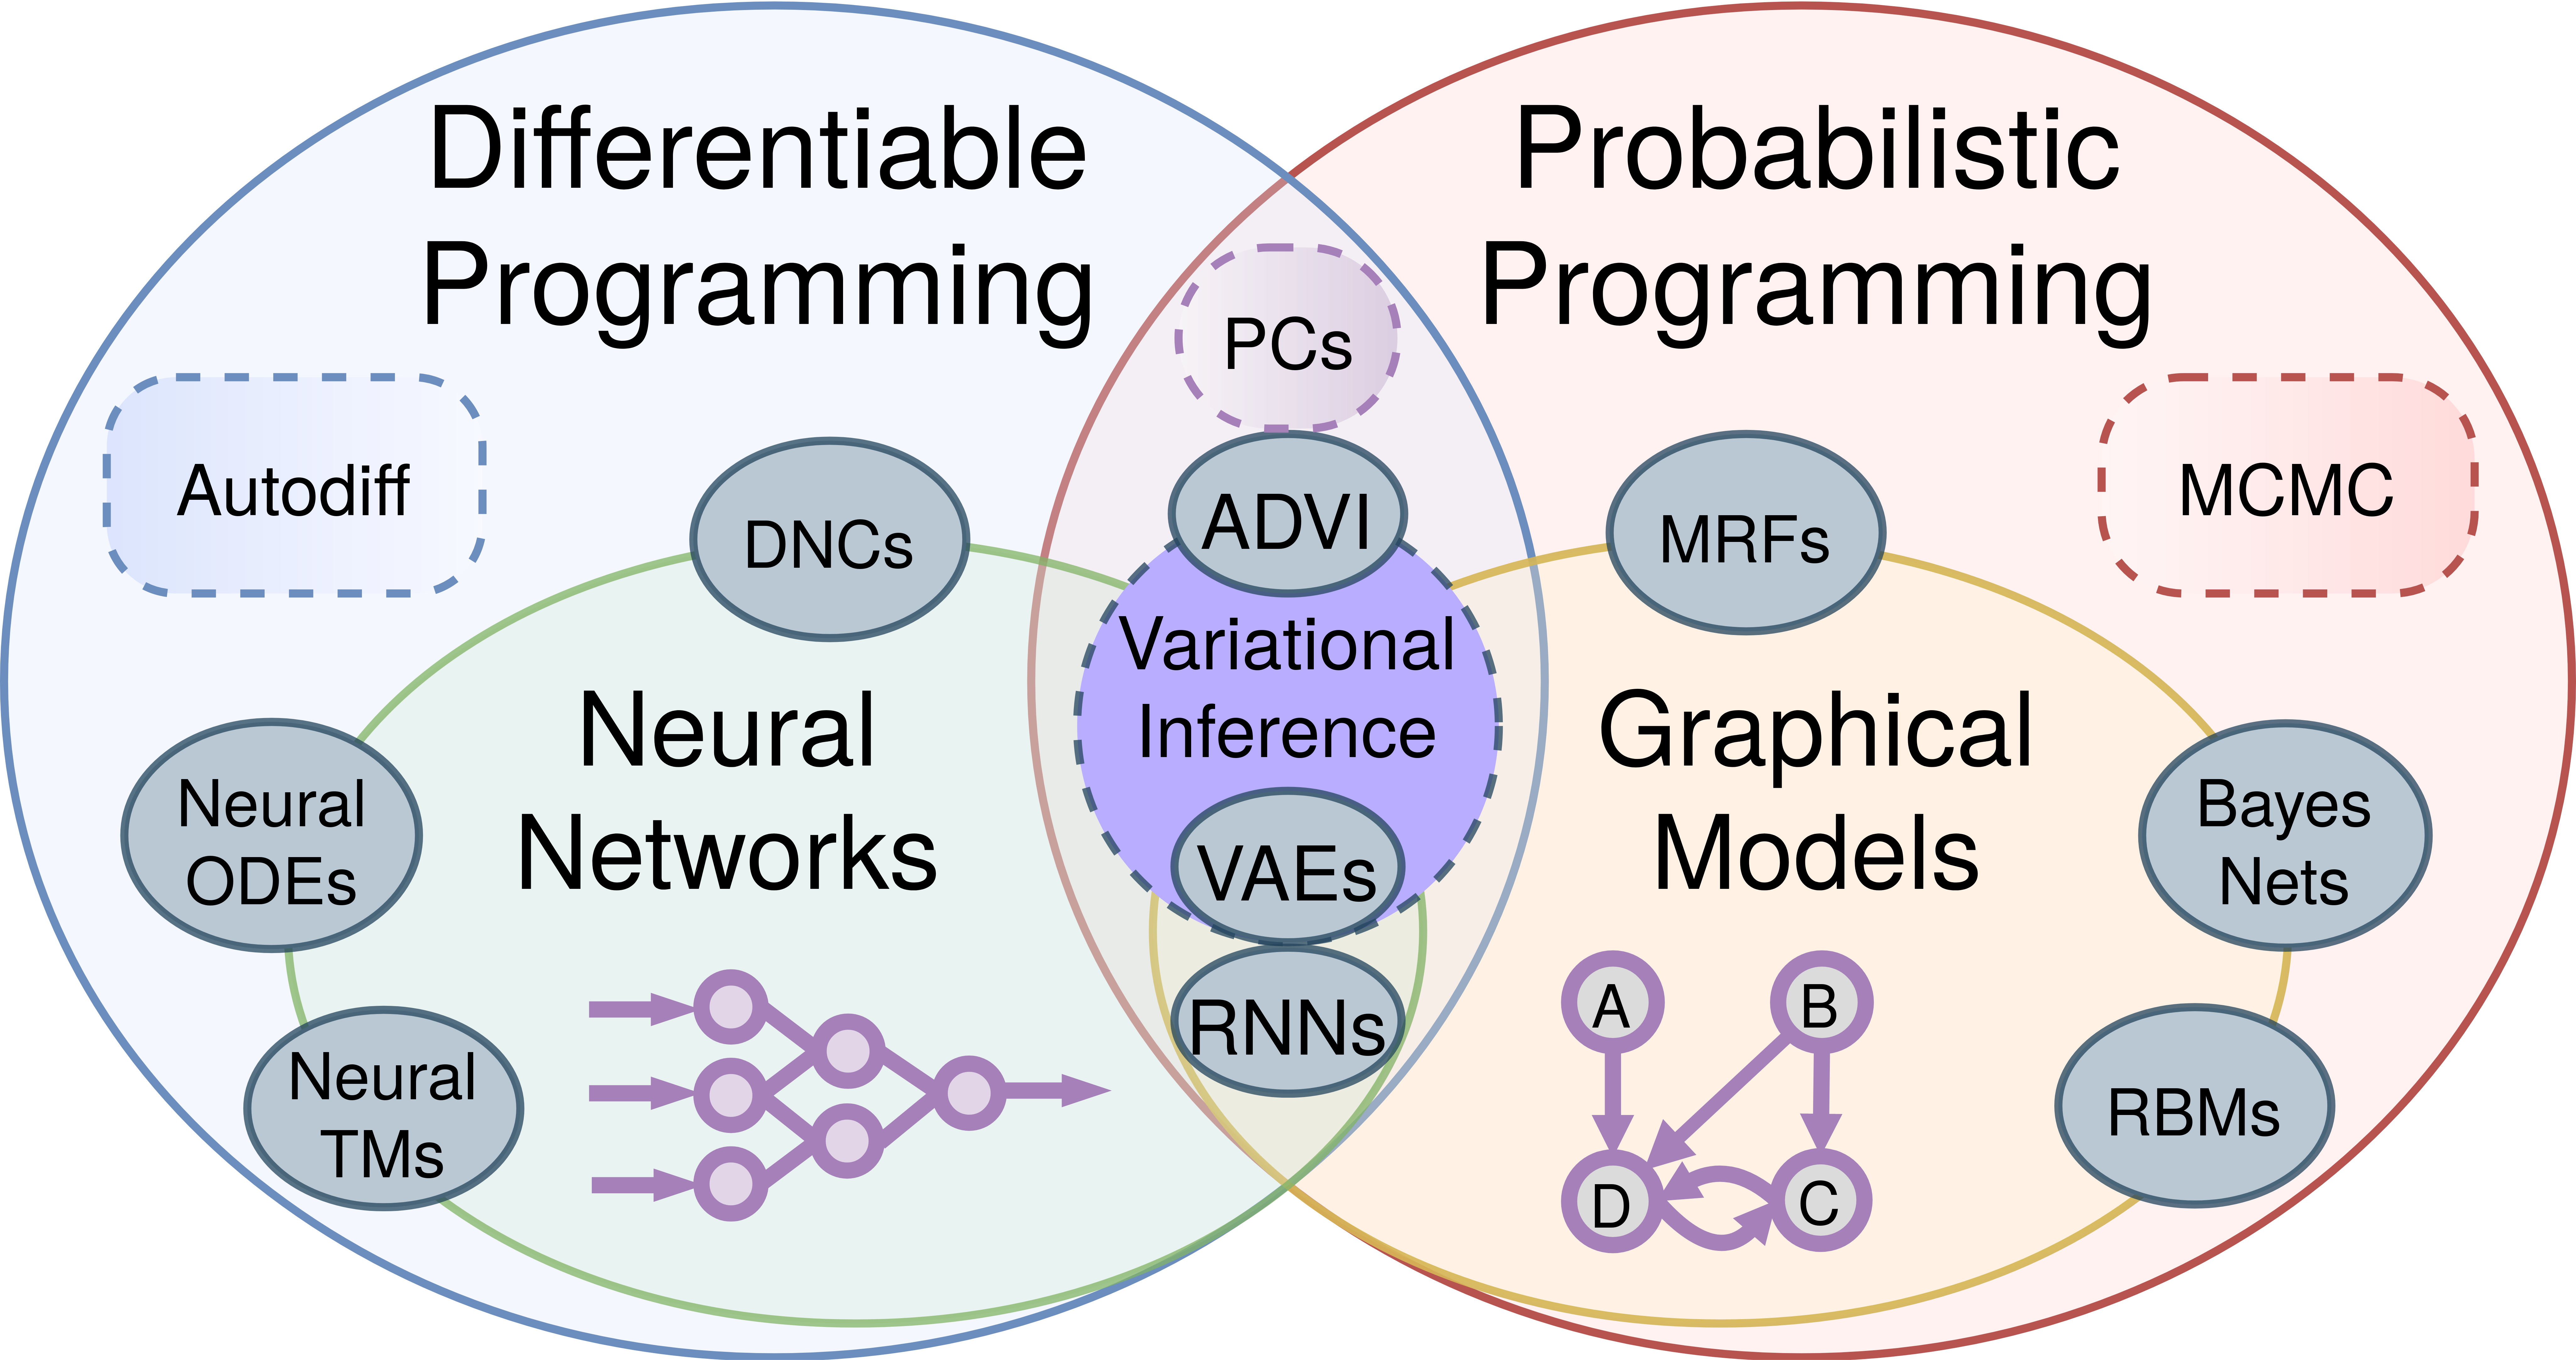
\includegraphics[width=0.90\textwidth]{../figures/diff_prob_prog.png}
    \caption{\textit{Differentiable programming} includes neural networks, but more broadly, arbitrary programs which use gradient-based optimization to approximate a loss function. \textit{Probabilistic programming}~\citep{tristan2014augur, carpenter2017stan, gorinova2018slicstan} is a generalization of probabilistic graphical models which uses Monte Carlo (MC) methods to approximate a density function.}
    \label{fig:diff_prob_prog}
\end{figure}

The renaissance of modern deep learning is widely attributed to progress in three research areas: algorithms, data and hardware. Among algorithms, most research has focused on deep learning architectures and representation learning. Equally important, arguably, is the role that automatic differentiation (AD) has played in facilitating the implementation of these ideas. Prior to the advent of general-purpose AD libraries such as \href{http://deeplearning.net/software/theano/}{Theano}, \href{https://pytorch.org/}{PyTorch} and \href{https://tensorflow.org/}{TensorFlow}, gradients had to be derived manually. The widespread adoption of AD software simplified and accelerated the pace of gradient-based machine learning, allowing researchers to build deeper network architectures and new learning representations. Some of these ideas in turn, formed the basis for new methods in AD, which continues to be an \href{http://www.autodiff.org}{active area} of research in the programming language and scientific computing communities.

A key aspect of the connectionist paradigm is gradient descent of a statistical loss function defined on a neural network with respect to its free parameters. For gradient descent to work, the representation must be differentiable almost everywhere. However, many representations are non-differentiable in their natural domain. For example, the structure of written language is not easily differentiable, as small changes to a word's symbolic form can cause sudden changes to its semantics~\citep{vanmerrienboer2018phd}. A key insight from representation learning is that many discrete data types can be mapped into a smoother latent space. For example, if we represent words as a vector of real numbers, $\mathbb R^N$, then it is possible to learn a mapping from words to $\mathbb R^N$ so that semantic relations between words (as defined by their statistical co-occurrence in large corpora) are geometrically preserved in vector space~\citep{pennington2014glove} -- words with similar meanings map to similar vectors. Many classes of discrete problems can be relaxed to continuous surrogates by learning such representations, or \textit{embeddings} in an unsupervised, or semi-supervised manner.

Around the same time, the deep learning community realized that perhaps strict differentiability was not so important all along. It was shown in practice, that computers using 8-bit floating point~\citep{wang2018training} and integer~\citep{wu2018training, jacob2018quantization} arithmetic are able to train neural networks without sacrificing performance. Strong assumptions like Lipschitz-continuity and $\beta$-smoothness once thought to be indispensable for gradient-based learning could be relaxed, as long as the noise introduced by quantization was negligible compared to stochastic gradient methods. In hindsight, this should have been less surprising, since all digital computers use discrete representations anyway and were capable of training neural networks for nearly half a century. This suggests strict differentiability was not as important as having a good metric. As long as the loss surface permits metric learning, gradient descent is surprisingly resilient to quantization.

As deep learning developed more applications, researchers observed that neural networks were part of a broader class of differentiable architectures which could bs structured in a manner not unlike computer programs. Hence the term \textit{differentiable programming}~\citep{olah2015neural, baydin2016differentiable, plotkin2018some} (DP) was born. Today, DP has many applications, from classical CS techniques like ranking and sorting~\citep{cuturi2019differentiable, blondel2020fast}, to protein folding~\citep{alquraishi2018end}, to physics engines~\citep{hu2019difftaichi, de2018end, degrave2016differentiable} and graphics rendering~\citep{loper2014opendr} to meta-learning~\citep{liu2018darts, chandra2019gradient}. These applications all have parameters that can be learned via gradient descent. To learn discrete relations without ad hoc embedding, additional techniques (\autoref{sec:future-work}), such as probabilistic programming, are likely needed. Various probabilistic programming languages including Stan~\citep{carpenter2017stan}, Pyro~\citep{bingham2019pyro}, PyMC4~\citep{kochurov2019pymc4} et al. have also emerged. As shown in \autoref{fig:diff_prob_prog}, these two fields have enjoyed many productive collaborations in recent years.

\section{Static and dynamic languages}

Most programs in machine learning and scientific computing are written in dynamic languages, such as Python. In contrast, most of the industry uses statically-typed languages~\citep{github}. According to some studies, type-related errors account for over 15\% of software bugs~\citep{gao2017type}. While the causality between defectiveness and static typing has not been conclusively established, dynamically-typed languages are seldom used for building safety-critical systems, and the majority of robotics applications~\citep{guenther2018serious} are written in statically-typed languages.

Static typing eliminates a broad class of runtime errors, allowing developers and tools to reason more carefully about the behavior of programs without needing to execute them. In addition to stronger syntax validation for general-purpose programming, a well-designed library in a strongly-typed language can eliminate domain-specific errors related to API misuse that would otherwise require documentation and code samples to avert, improving usability and reducing maintenance. Furthermore, strong type systems allow IDEs to provide more precise static analysis tools, such as relevant autocompletion, source code navigation, and earlier detection of runtime errors.

One common objection to using strongly-typed languages is the additional burden of manual type annotation~\citep{ore2018assessing}. While early type-safe languages like C++ and Java required programmers to exhaustively annotate function and variable declarations, with judicious use of type inference in modern languages like Kotlin, Scala, Rust et al., most type signatures can be safely omitted and easily recovered from the surrounding context. Type inference enables modern languages to offer the brevity of dynamically-typed languages with the safety of static type checking.

\section{Imperative and functional languages}

Most programs today are written in the imperative style, due the prevalence of the Turing machine and von Neumann architecture~\citep{backus2007can}. $\lambda$-calculus provides an equivalent\footnote{In the sense that the Turing Machine and $\lambda$-calculus are both Turing complete.} language for computing, which we argue, is a more appropriate notation for expressing mathematical functions and computing their derivatives. In imperative programming the sole purpose of using a function is to pass it values, and there is no way to refer to a function without doing so. More troubling in the case of AD, is that imperative programs have mutable state, which requires taking extra precautions when computing their derivatives.

The mathematical notion for function composition is a first-class citizen in functional programming. Just like in calculus, to take the derivative of a program composed with another program, we simply apply the chain rule (\autoref{sec:automatic-differentiation}). Since there is no mutable state in FP, no exotic data structures or compiler tricks are required.

For example, consider the vector function $f(l_1, l_2) = l_1 \cdot l_2$, seen in \autoref{fig:fp_vs_ip}. Imperative programs, by allowing mutation, are effectively destroying intermediate information. In order to recover the computation graph for reverse-mode AD, we either need to override the assignment operator, or use a tape to store the intermediate values. In pure functional programming, mutable variables do not exist, which makes our lives much easier.

\begin{figure}[t]
    \centering
    \begin{tabular}{|l|l|}
        \hline
        Imperative & Functional \\
        \hline
{\begin{lstlisting}[style=barelisting, linewidth=5.7cm, numbers=left]
fun dot(l1, l2) {
    if (len(l1) != len(l2))
        return error
    var sum = 0
    for(i in 0 to len(l1))
        sum += l1[i] * l2[i]
    return sum
}
\end{lstlisting}}
        &
{\begin{lstlisting}[style=barelisting, linewidth=6.5cm, numbers=none]
fun dot(l1, l2) {
    return if (len(l1) != len(l2))
        error
    else if (len(l1) == 0) 0
    else
        head(l1) * head(l2) +
        dot(tail(l1), tail(l2))
}
\end{lstlisting}}
        \\
        \hline
    \end{tabular}
    \caption{Two equivalent programs, both implementing the function $f(l_1, l_2) = l_1 \cdot l_2$.}
    \label{fig:fp_vs_ip}
\end{figure}

Functional programming lets Kotlin$\nabla$ use the same abstraction for representing mathematical functions and programming functions. All functions in Kotlin$\nabla$ are pure functions, composed of expressions forming a data-flow graph (DFG). An expression is simply a \inline{Function}, which is only evaluated when invoked with numerical values, e.g. \inline{z(0, 0)}. In this way, Kotlin$\nabla$ is similar to other graph-based frameworks like \href{http://deeplearning.net/software/theano/extending/graphstructures.html}{Theano} and \href{https://www.tensorflow.org/guide/graphs}{TensorFlow}.

\section{Kotlin}\label{sec:kotlin}

When programming in a statically-typed language, a common question one might ask the compiler is, ``Given a value, \inline{x}, can \inline{x} be assigned to a variable of type \inline{Y}?'' (e.g. type checking \inline{x instanceof Y}) In Java, this question turns out to be \href{http://io.livecode.ch/learn/namin/unsound}{ill-posed}~\citep{amin2016java} and undecidable~\citep{grigore2017java} in the general case. It is possible to construct a Java program in which the answer is ``yes'' regardless of \inline{Y}, or for which an answer cannot always be determined in finite time. Undecidability is not necessarily a showstopper, but Java's unsoundness is more critical and unclear how to fix, even though it rarely occurs in practice.

Kotlin is a statically-typed language that is well-suited for building cross-platform applications, with compiler support for JVM, JavaScript and native targets. Unlike most programming languages, Kotlin was designed with IDE support from the outset, and has gained some traction in the JVM ecosystem due to its ergonomics. Kotlin's type system~\citep{tate2013mixed} is strictly \href{https://kotlinlang.org/docs/reference/generics.html#variance}{less expressive}, but fully interoperable with Java's. It is unknown whether the same issues which affect Java's type system are present in Kotlin's, but interoperability with Java has broadened its adoption and remains a key usability feature of the language.

In this work, we make use of several language features unique to Kotlin, such as first-class functions (\autoref{sec:first-class-functions}), extension functions (\autoref{sec:extension-functions}), operator overloading (\autoref{sec:operator-overloading}), and algebraic data types (\autoref{sec:adts}). Furthermore, we make heavy use of Kotlin's \href{https://kotlinlang.org/docs/reference/type-safe-builders.html}{DSL support} to implement shape-safe array programming. Together, these language features provide a concise, flexible and type-safe platform for mathematical programming.

\section{Kotlin\textorpdfstring{$\nabla$}}\label{sec:kotlingrad}

Prior work has demonstrated the possibility of encoding a deterministic context free (DCF) language in the Java type system as a \textit{fluent interface}~\citep{gil2016formal, nakamaru2017silverchain}. This result was strengthened to prove Java's type system is Turing complete (TC)~\citep{grigore2017java}, which enables us to perform shape checking and inference on array programs written in Java. Kotlin is a Java descendant which is at least DCF at the type level. Kotlin$\nabla$, an embedded DSL in the Kotlin language is TC at the value level and DCF at the type level. A similar approach is feasible in most languages with generic types.

Differentiable programming has a rich history among dynamic languages like Python, Lua and JavaScript, with early implementations including projects like \href{http://deeplearning.net/software/theano/}{Theano}~\citep{bergstra2010theano}, \href{http://torch.ch/}{Torch}~\citep{collobert2002torch}, and \href{https://tensorflow.org/}{TensorFlow}~\citep{abadi2016tensorflow}. Similar ideas have been implemented in functional languages such as Scheme (\href{https://github.com/Functional-AutoDiff/STALINGRAD}{Stalin$\nabla$}~\citep{pearlmutter2008using}), and statically-typed languages like F\# (\href{https://diffsharp.github.io/DiffSharp/}{DiffSharp}~\citep{baydin2015diffsharp}) and \href{https://www.tensorflow.org/swift}{Swift}~\citep{lattner2018tensorflow}. However, the majority of existing automatic differentiation (AD) libraries use a loosely-typed DSL, and few offer shape-safe tensor operations in a widely-used programming language.

Existing AD implementations for the JVM include \href{https://feiwang3311.github.io/Lantern/}{Lantern}~\citep{wang2018demystifying}, \href{https://tongfei.me/nexus/}{Nexus}~\citep{chen2017typesafe} and \href{https://github.com/ThoughtWorksInc/DeepLearning.scala}{DeepLearning.scala}~\citep{yang2018dl4s}, however these are Scala-based and do not interoperate with other JVM languages. Kotlin$\nabla$ is fully interoperable with vanilla Java, enabling broader adoption in neighboring languages. To our knowledge, Kotlin has no prior AD implementation. However, the language has several useful features for implementing a native AD framework. Kotlin$\nabla$ primarily relies on the following language features:

\begin{itemize}
    \item \textbf{Operator overloading and infix functions} allow a concise notation for defining arithmetic operations on tensor-algebraic structures, i.e.\ groups, rings and fields.
    \item \textbf{$\mathbf{\lambda}$-functions} support functional programming, following~\citet{pearlmutter2008reverse, pearlmutter2008using, siskind2008nesting, elliott2009beautiful, elliott2018simple}, et al.
    \item \textbf{Extension functions} support extending classes with new fields and methods which can be exposed to external callers without requiring sub-classing or inheritance.
\end{itemize}

\begin{figure}
    \centering
    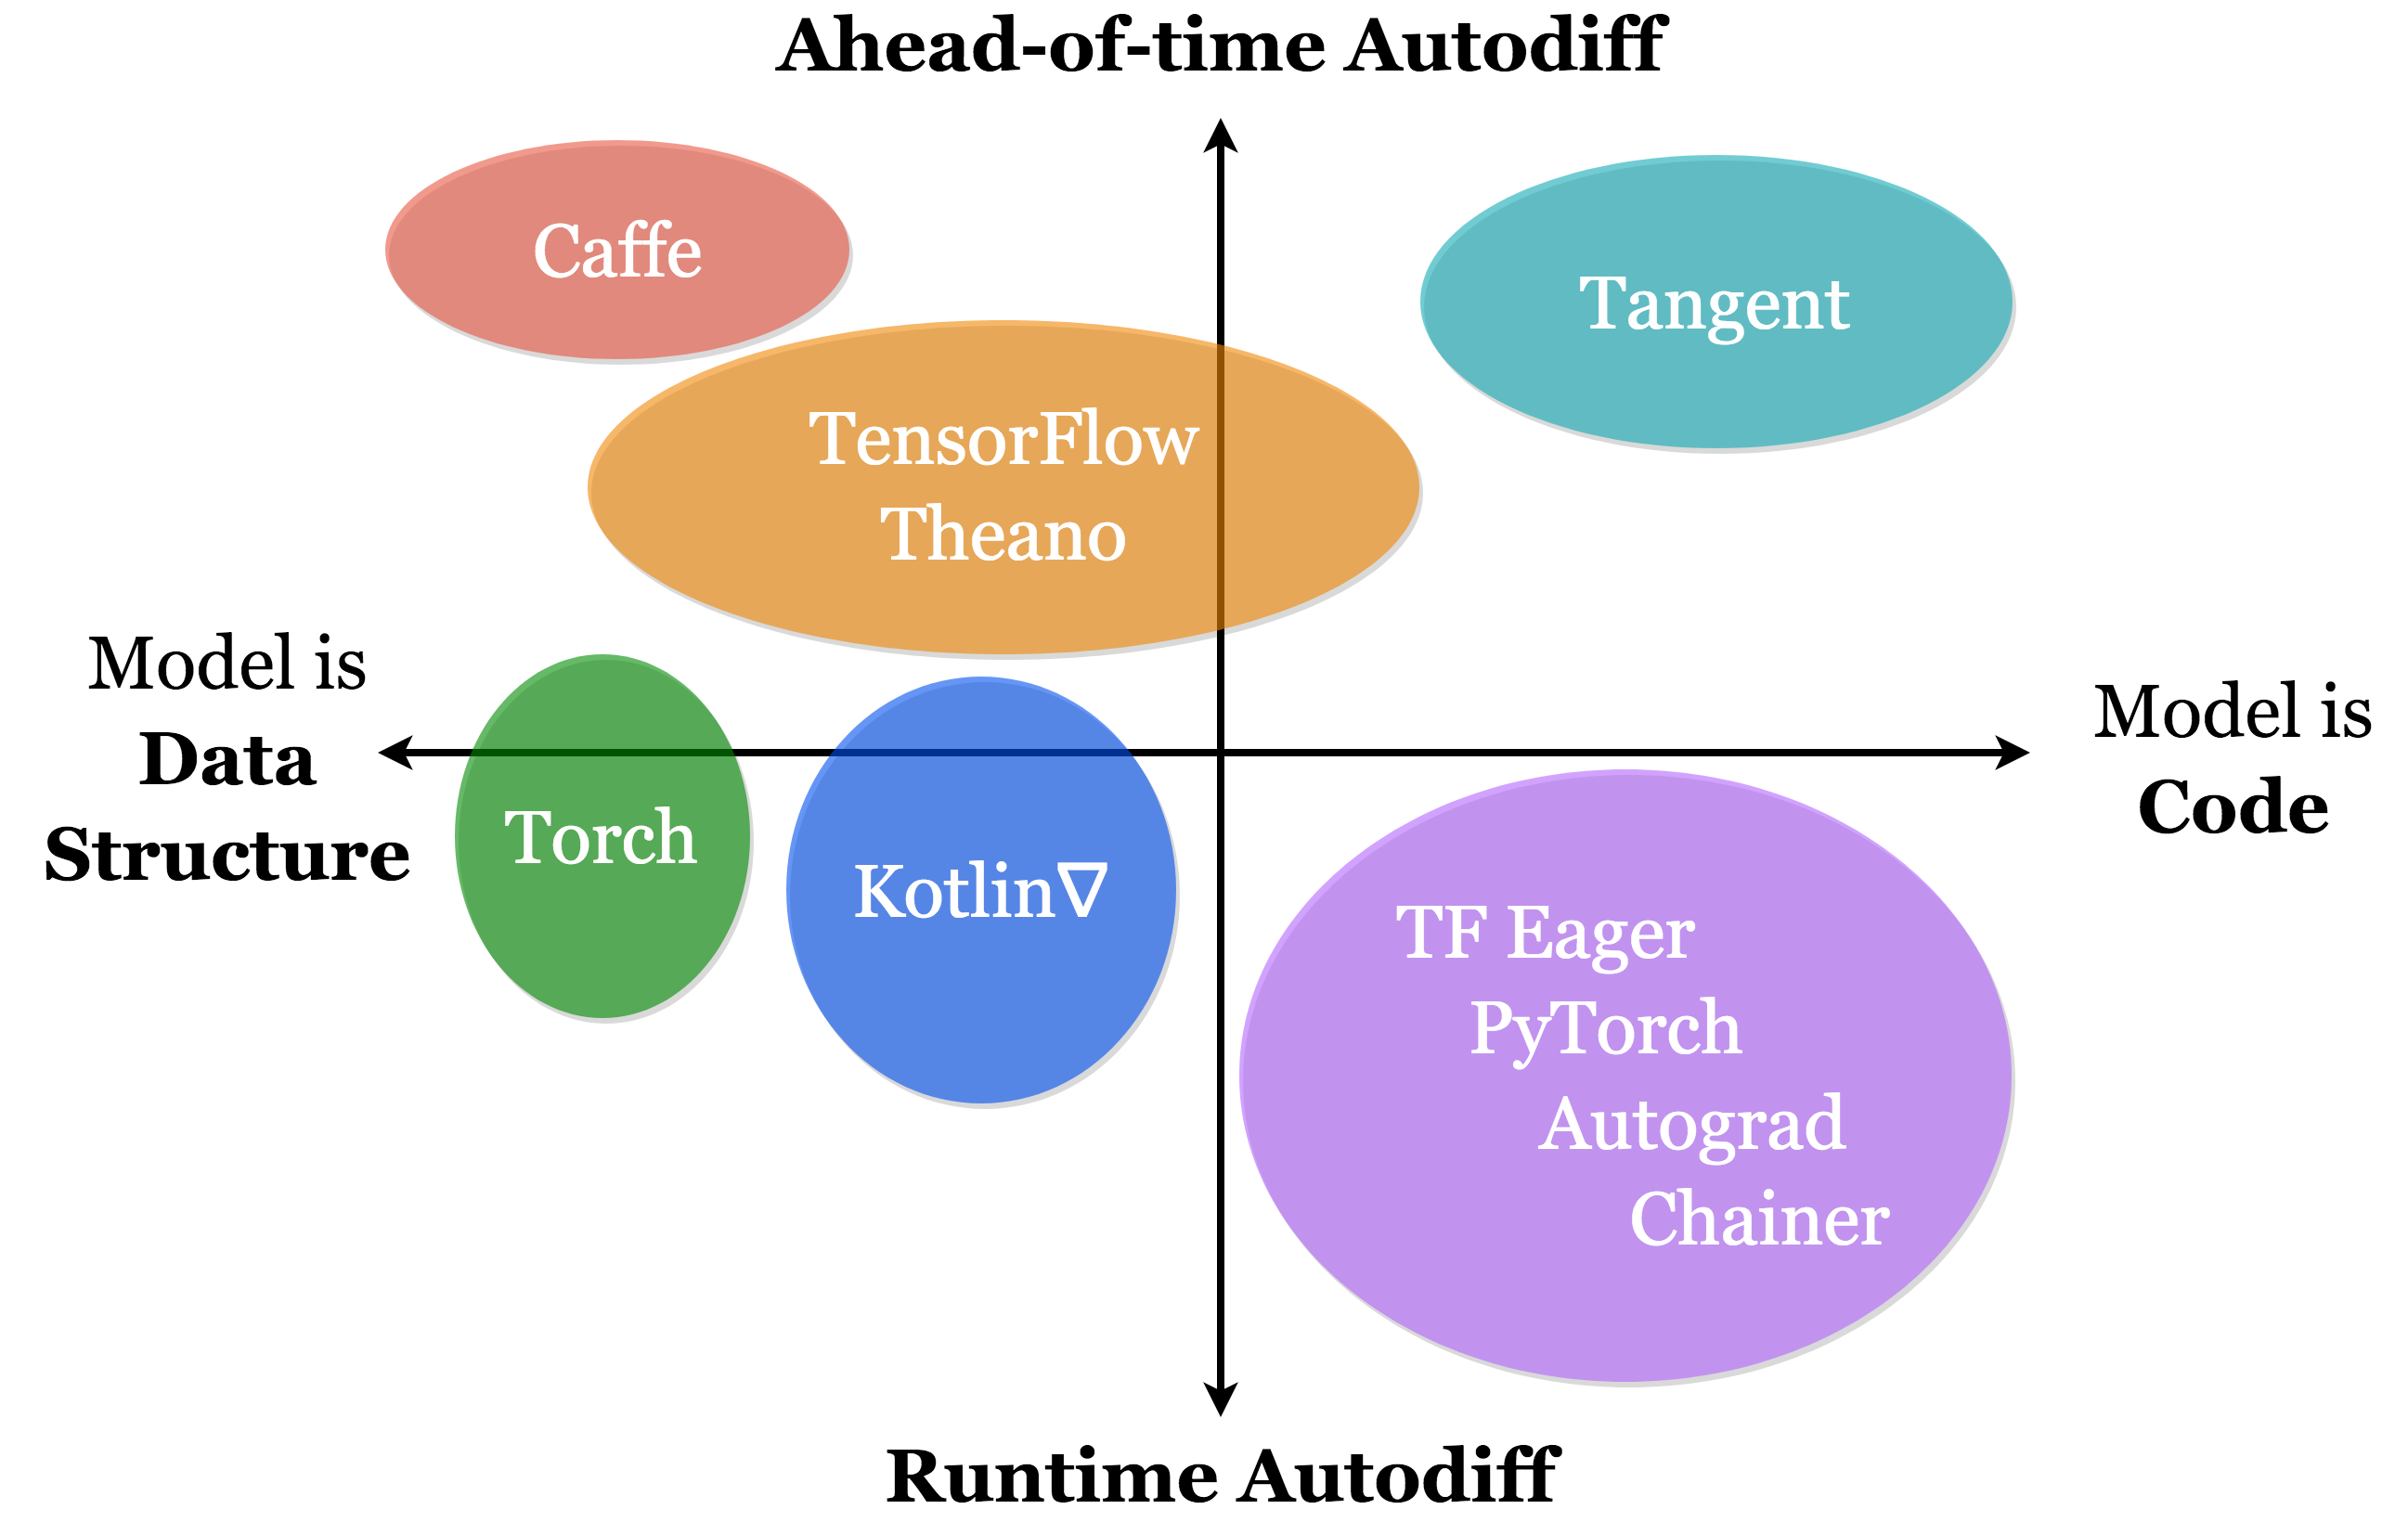
\includegraphics[width=0.70\textwidth]{../figures/kotlingrad_diagram.png}
    \caption{Adapted from~\citet{van2018tangent}. Kotlin$\nabla$ models are data structures, constructed by an embedded DSL, eagerly optimized, and lazily evaluated.}
    \label{fig:kotlingrad_digram}
\end{figure}

Kotlin$\nabla$ models are embedded domain-specific languages (eDSLs). These languages may appear and behave unlike the host language, but are really just carefully disguised functions for building an abstract syntax tree (AST). Often these ASTs represent simple state machines, but are also used to embed a programming language. Popular examples include \href{https://docs.microsoft.com/en-us/dotnet/framework/data/adonet/sql/linq/}{SQL/LINQ}~\citep{meijer2006linq}, \href{http://stanford-ppl.github.io/Delite/optiml/}{OptiML}~\citep{sujeeth2011optiml} and other fluent interfaces~\citep{fowler05fluent}. In a sufficiently expressive host language, one can implement any language as a library, without the need to write a lexer, parser, compiler or interpreter. And with proper typing, users will receive code completion and static analysis from their favorite developer tools. Functional languages are often suitable host languages~\citep{elliott2003compiling,rompf2010lightweight}, perhaps owing to the notion of code as data.

\section{Usage}

Kotlin$\nabla$ allows users to implement differentiable programs by composing expressions. Consider the following Kotlin$\nabla$ program with two inputs and one output:
%
\begin{figure}[H] \label{fig:basic_kotlingrad}
\begin{unbreakablekotlin}
with(DoublePrecision) { // Uses double precision numerics for evaluation
  val x by Var() // Declare immutable variables (these variables are
  val y by Var() // just symbolic constructs used for differentiation)
  val z = sin(10 * (x * x + pow(y, 2))) / 10 // Lazily evaluated
  val dz_dx = d(z) / d(x) // Supports Leibniz notation(*@~\citep{christianson2012leibniz}@*)
  val d2z_dxdy = d(dz_dx) / d(y) // Mixing higher order partials
  val d3z_d2xdy = grad(d2z_dxdy)[x] // Equivalent to d(f)/d(x)
  plot3D(d3z_d2xdy, -1.0, 1.0) // Plot in 3-space (-1 < x, y, z < 1)
}
\end{unbreakablekotlin}
%    \centering $z = \sin{\big(10(x*x + y^2)\big)} / 10$, \texttt{plot}$\Big\left(\frac{\partial^{3z}}{\partial{x^2}\partial{y}}\Big\right)$ \\
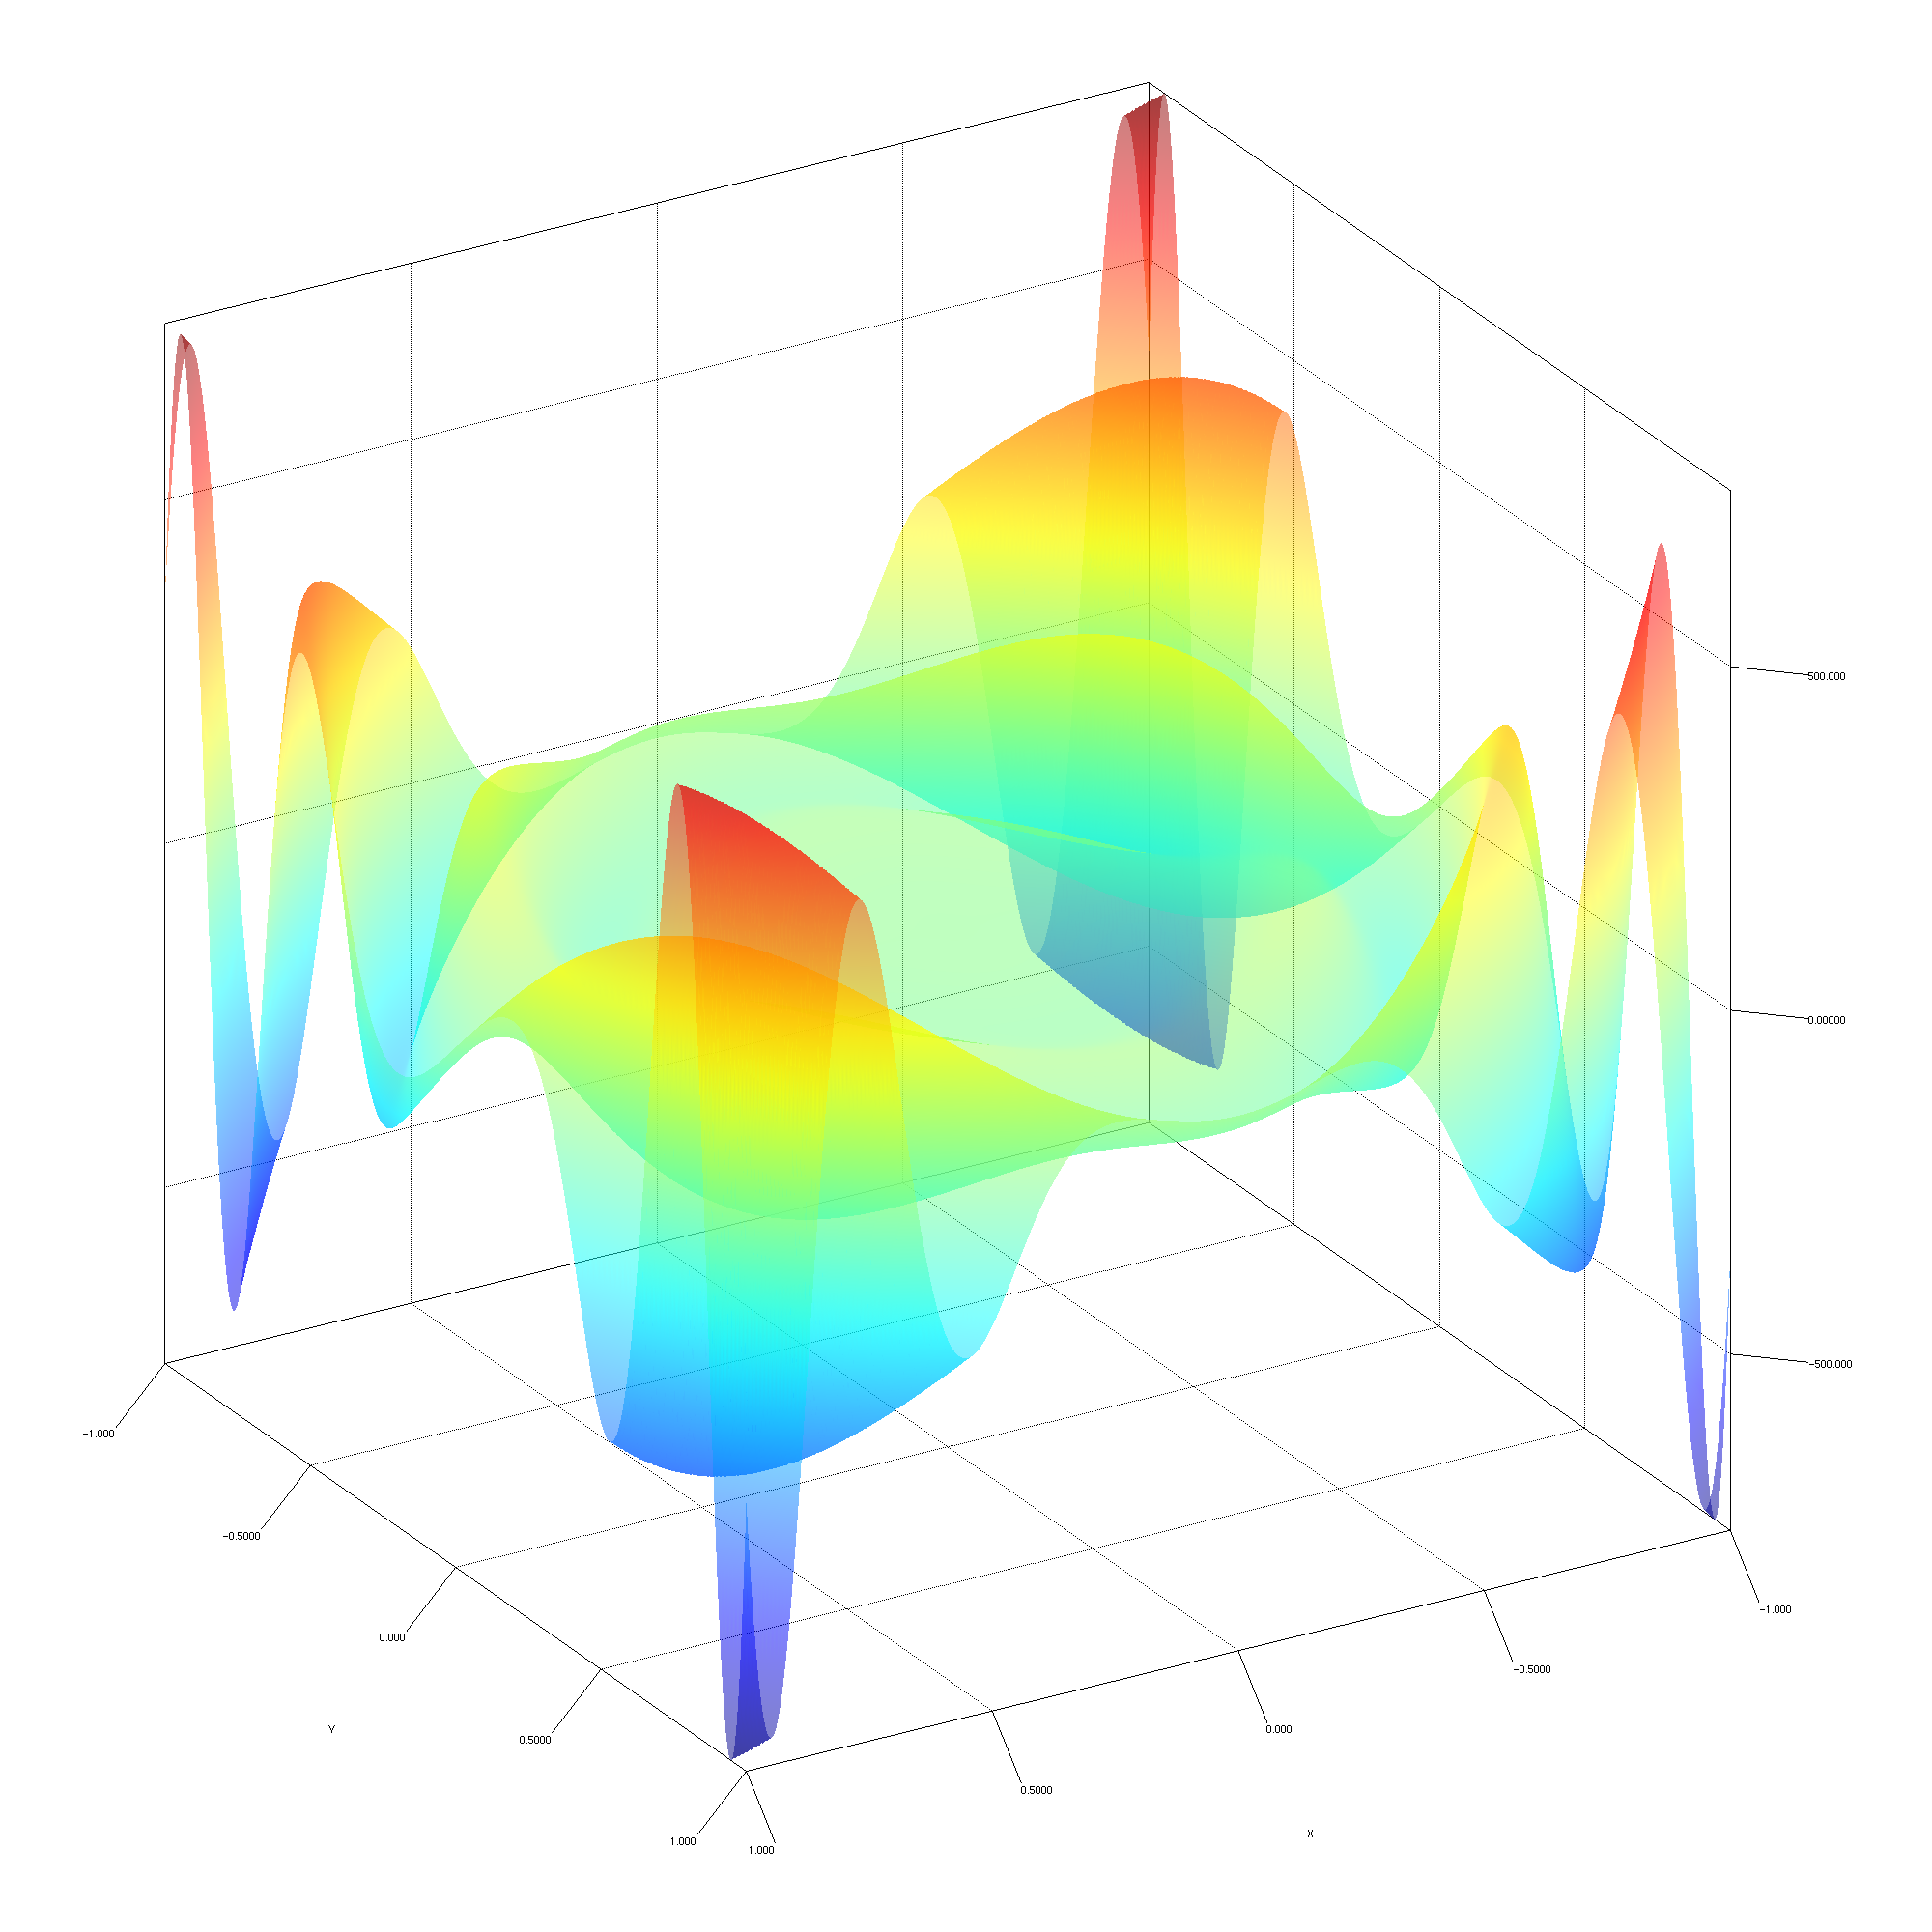
\includegraphics[scale=0.43]{../figures/plot_result.png}
\end{figure}
%
Above, we define a function with two variables and take a series of partial derivatives with respect to each variable. Expressions are lazily evaluated inside a numerical context, which may be imported on a per-file basis or lexically scoped for finer-grained control over the runtime behavior. The function is numerically evaluated on the interval $(-1, 1)$ in each dimension and rendered in 3-space. For a complete grammar, please refer to~\autoref{sec:kg_grammar}.
% We can also plot higher dimensional manifolds (e.g.\ the loss surface of a neural network), projected into four dimensions, and rendered in three, where one axis is represented by time.
%
\begin{figure}
%\begin{unbreakablekotlin}
%val z = sin(10 * (x * x + pow(y, 2))) / 10 // Does not perform calculation
%\end{unbreakablekotlin}
    \begin{unbreakablekotlin}
        val t = (1 + x * 2 + z / y).d(y).d(x) + z / y * 3 - 4 * (y pow y).d(y)
    \end{unbreakablekotlin}
\end{figure}
\vspace{-40pt}
\begin{figure}
    \centering
%\begin{tikzpicture}[grow=left]
%    \tikzset{level distance=60pt}
%    \Tree [.$\div$ [.\inline{sin} [.$\times$ \inline{10} [.$+$ [.$\times$ \inline{\textbf{x}} \inline{\textbf{x}} ] [.\inline{pow} \inline{\textbf{y}} \inline{2} ] ] ] ] \inline{10} ]
%\end{tikzpictre}
%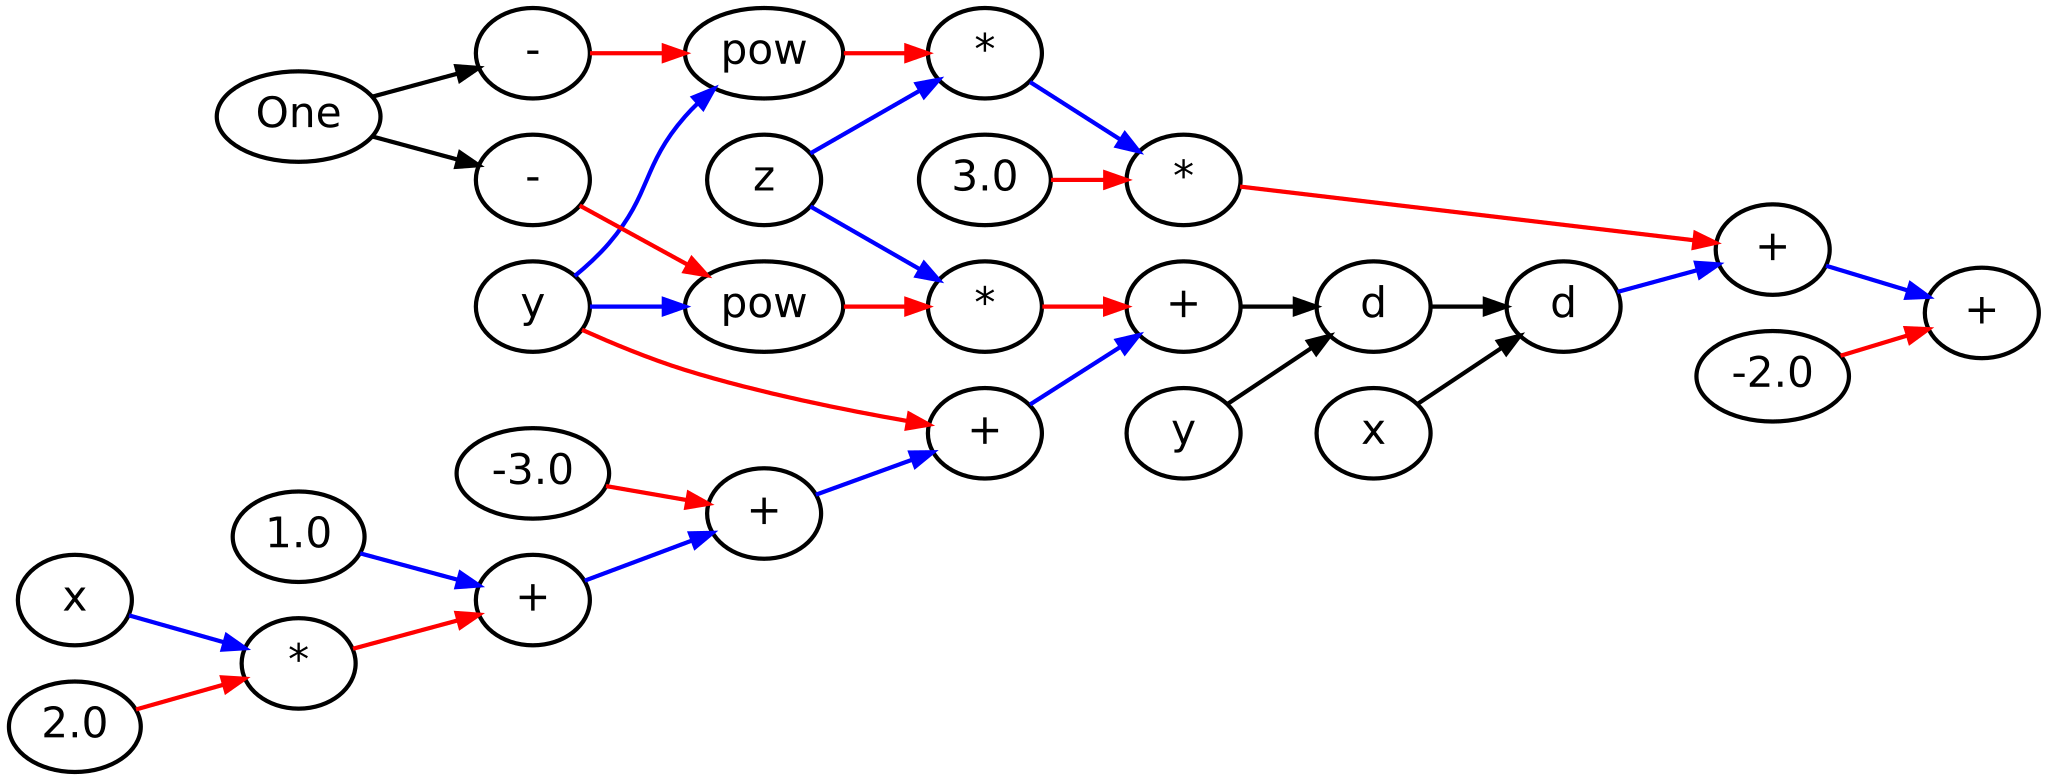
\includegraphics[scale=0.60]{../figures/dataflow.png}
    \digraph[scale=0.5]{dfg} { graph ["rankdir"="LR","bgcolor"="transparent"]; "209813603" ["color"="black","fontcolor"="black","fontname"="Helvetica","fontsize"="20","style"="setlinewidth(2)","label"="+"]; "659748578" ["color"="black","fontcolor"="black","fontname"="Helvetica","fontsize"="20","style"="setlinewidth(2)","label"="+"]; "483422889" ["color"="black","fontcolor"="black","fontname"="Helvetica","fontsize"="20","style"="setlinewidth(2)","label"="d"]; "1277181601" ["color"="black","fontcolor"="black","fontname"="Helvetica","fontsize"="20","style"="setlinewidth(2)","label"="d"]; "488970385" ["color"="black","fontcolor"="black","fontname"="Helvetica","fontsize"="20","style"="setlinewidth(2)","label"="+"]; "93122545" ["color"="black","fontcolor"="black","fontname"="Helvetica","fontsize"="20","style"="setlinewidth(2)","label"="+"]; "1239731077" ["color"="black","fontcolor"="black","fontname"="Helvetica","fontsize"="20","style"="setlinewidth(2)","label"="1.0"]; "249515771" ["color"="black","fontcolor"="black","fontname"="Helvetica","fontsize"="20","style"="setlinewidth(2)","label"="*"]; "x" ["color"="black","fontcolor"="black","fontname"="Helvetica","fontsize"="20","style"="setlinewidth(2)"]; "1627960023" ["color"="black","fontcolor"="black","fontname"="Helvetica","fontsize"="20","style"="setlinewidth(2)","label"="2.0"]; "1811044090" ["color"="black","fontcolor"="black","fontname"="Helvetica","fontsize"="20","style"="setlinewidth(2)","label"="*"]; "z" ["color"="black","fontcolor"="black","fontname"="Helvetica","fontsize"="20","style"="setlinewidth(2)"]; "940060004" ["color"="black","fontcolor"="black","fontname"="Helvetica","fontsize"="20","style"="setlinewidth(2)","label"="*"]; "1945604815" ["color"="black","fontcolor"="black","fontname"="Helvetica","fontsize"="20","style"="setlinewidth(2)","label"="*"]; "328638398" ["color"="black","fontcolor"="black","fontname"="Helvetica","fontsize"="20","style"="setlinewidth(2)","label"="pow"]; "y" ["color"="black","fontcolor"="black","fontname"="Helvetica","fontsize"="20","style"="setlinewidth(2)"]; "1121172875" ["color"="black","fontcolor"="black","fontname"="Helvetica","fontsize"="20","style"="setlinewidth(2)","label"="pow"]; "1644443712" ["color"="black","fontcolor"="black","fontname"="Helvetica","fontsize"="20","style"="setlinewidth(2)","label"="pow"]; "745160567" ["color"="black","fontcolor"="black","fontname"="Helvetica","fontsize"="20","style"="setlinewidth(2)","label"="d"]; "391447681" ["color"="black","fontcolor"="black","fontname"="Helvetica","fontsize"="20","style"="setlinewidth(2)","label"="*"]; "1308927845" ["color"="black","fontcolor"="black","fontname"="Helvetica","fontsize"="20","style"="setlinewidth(2)","label"="-"]; "440434003" ["color"="black","fontcolor"="black","fontname"="Helvetica","fontsize"="20","style"="setlinewidth(2)","label"="-"]; "1" ["color"="black","fontcolor"="black","fontname"="Helvetica","fontsize"="20","style"="setlinewidth(2)","label"="One"]; "1595953398" ["color"="black","fontcolor"="black","fontname"="Helvetica","fontsize"="20","style"="setlinewidth(2)","label"="-"]; "1277181601{color=black, fontcolor=black, fontname=Helvetica, fontsize=20, style=setlinewidth(2)}->" ["color"="black","fontcolor"="black","fontname"="Helvetica","fontsize"="20","style"="setlinewidth(2)","label"="y"]; "483422889{color=black, fontcolor=black, fontname=Helvetica, fontsize=20, style=setlinewidth(2)}->" ["color"="black","fontcolor"="black","fontname"="Helvetica","fontsize"="20","style"="setlinewidth(2)","label"="x"]; "1684106402" ["color"="black","fontcolor"="black","fontname"="Helvetica","fontsize"="20","style"="setlinewidth(2)","label"="3.0"]; "403424356" ["color"="black","fontcolor"="black","fontname"="Helvetica","fontsize"="20","style"="setlinewidth(2)","label"="4.0"]; "745160567{color=black, fontcolor=black, fontname=Helvetica, fontsize=20, style=setlinewidth(2)}->" ["color"="black","fontcolor"="black","fontname"="Helvetica","fontsize"="20","style"="setlinewidth(2)","label"="y"]; "659748578" -> "209813603" ["color"="blue","arrowhead"="normal","style"="setlinewidth(2)"]; "483422889" -> "659748578" ["color"="blue","arrowhead"="normal","style"="setlinewidth(2)"]; "1277181601" -> "483422889" ["color"="black","arrowhead"="normal","style"="setlinewidth(2)"]; "488970385" -> "1277181601" ["color"="black","arrowhead"="normal","style"="setlinewidth(2)"]; "93122545" -> "488970385" ["color"="blue","arrowhead"="normal","style"="setlinewidth(2)"]; "1239731077" -> "93122545" ["color"="blue","arrowhead"="normal","style"="setlinewidth(2)"]; "249515771" -> "93122545" ["color"="red","arrowhead"="normal","style"="setlinewidth(2)"]; "x" -> "249515771" ["color"="blue","arrowhead"="normal","style"="setlinewidth(2)"]; "1627960023" -> "249515771" ["color"="red","arrowhead"="normal","style"="setlinewidth(2)"]; "1811044090" -> "488970385" ["color"="red","arrowhead"="normal","style"="setlinewidth(2)"]; "z" -> "1811044090" ["color"="blue","arrowhead"="normal","style"="setlinewidth(2)"]; "z" -> "940060004" ["color"="blue","arrowhead"="normal","style"="setlinewidth(2)"]; "940060004" -> "1945604815" ["color"="blue","arrowhead"="normal","style"="setlinewidth(2)"]; "1945604815" -> "659748578" ["color"="red","arrowhead"="normal","style"="setlinewidth(2)"]; "328638398" -> "1811044090" ["color"="red","arrowhead"="normal","style"="setlinewidth(2)"]; "y" -> "328638398" ["color"="blue","arrowhead"="normal","style"="setlinewidth(2)"]; "y" -> "1121172875" ["color"="blue","arrowhead"="normal","style"="setlinewidth(2)"]; "y" -> "1644443712" ["color"="blue","arrowhead"="normal","style"="setlinewidth(2)"]; "y" -> "1644443712" ["color"="red","arrowhead"="normal","style"="setlinewidth(2)"]; "1121172875" -> "940060004" ["color"="red","arrowhead"="normal","style"="setlinewidth(2)"]; "1644443712" -> "745160567" ["color"="black","arrowhead"="normal","style"="setlinewidth(2)"]; "745160567" -> "391447681" ["color"="red","arrowhead"="normal","style"="setlinewidth(2)"]; "391447681" -> "1308927845" ["color"="black","arrowhead"="normal","style"="setlinewidth(2)"]; "1308927845" -> "209813603" ["color"="red","arrowhead"="normal","style"="setlinewidth(2)"]; "440434003" -> "328638398" ["color"="red","arrowhead"="normal","style"="setlinewidth(2)"]; "1" -> "440434003" ["color"="black","arrowhead"="normal","style"="setlinewidth(2)"]; "1" -> "1595953398" ["color"="black","arrowhead"="normal","style"="setlinewidth(2)"]; "1595953398" -> "1121172875" ["color"="red","arrowhead"="normal","style"="setlinewidth(2)"]; "1277181601{color=black, fontcolor=black, fontname=Helvetica, fontsize=20, style=setlinewidth(2)}->" -> "1277181601" ["color"="black","arrowhead"="normal","style"="setlinewidth(2)"]; "483422889{color=black, fontcolor=black, fontname=Helvetica, fontsize=20, style=setlinewidth(2)}->" -> "483422889" ["color"="black","arrowhead"="normal","style"="setlinewidth(2)"]; "1684106402" -> "1945604815" ["color"="red","arrowhead"="normal","style"="setlinewidth(2)"]; "403424356" -> "391447681" ["color"="blue","arrowhead"="normal","style"="setlinewidth(2)"]; "745160567{color=black, fontcolor=black, fontname=Helvetica, fontsize=20, style=setlinewidth(2)}->" -> "745160567" ["color"="black","arrowhead"="normal","style"="setlinewidth(2)"]; }

    \caption{Implicit DFG constructed by the original expression, shown above.}
    \label{lst:edsl}
\end{figure}\\\\

\section{Type systems}\label{sec:type-systems}

Early work in type-safe dimension analysis can be found in \citet{kennedy1994dimension, kennedy1996programming} which uses types to encode dimensionality and prevent common bugs related to dimension mismatch from arising, and was later realized in the F\# language~\citep{kennedy2010types}. \citet{jay1996shape}, \citet{rittri1995dimension}, and \citet{zenger1997indexed} explore the application of dimension types for linear algebra. More recently, \citet{kiselyov2005number, kiselyov2010fun} and \citet{griffioen2015type}, show how to manipulate arrays in more complex ways. With the resurgence of interest in tensor algebra and array programming, \citet{chen2017typesafe} and \citet{rink2018modeling} demonstrate how to encode shape-safety for tensor algebra in various type systems.

The problem we attempt to solve can be summarized as follows. Given two values \inline{x} and \inline{y}, and operator \inline{\$}, how do we determine whether the expression \inline{z = x \$ y} is valid, and if so, what is the result type of \inline{z}? For matrix multiplication, when \inline{x} $\in \mathbb{R}^{m \times n}$ and \inline{y} $\in \mathbb{R}^{n \times p}$, the expression is well-typed and we can infer \inline{z} $\in \mathbb{R}^{m \times p}$. More generally, we would like to infer the type of \inline{z} for some operator \inline{@} $: (\mathbb{R}^\mathbf{a}, \mathbb{R}^\mathbf{b}) \rightarrow \mathbb{R}^\mathbf{c}$ where $\mathbf{a} \in \mathbb{N}^q, \mathbf{b} \in \mathbb{N}^r, \mathbf{c} \in \mathbb{N}^s$ and $q, r, s \in \mathbb{N}$. For many linear algebra operations such as matrix multiplication, $\mathcal{S}(\mathbf a, \mathbf b) \stackrel{?}{=} \mathbf c$ is computable in $\mathcal{O}(1)$ -- we can simply check the inner dimensions for equivalence ($\mathbf{a}_2 \stackrel{?}{=} \mathbf{b}_1$).

Shape checking multidimensional array operators is not always decidable. For arbitrary shape functions $\mathcal{S}(\mathbf{a}, \mathbf{b})$, checking $\mathcal{S}(\mathbf{a}, \mathbf{b}) \stackrel{?}{=} \mathbf{c}$ requires a Turing machine. If $\mathcal{S}$ uses the multiplication operator, as in the case of convolutional arithmetic~\citep{dumoulin2016guide}, shape inference becomes equivalent to Peano arithmetic, which is undecidable~\citep{godel1931formal}. Addition, subtraction, indexing and comparison of integers are all decidable in Presburger arithmetic~\citep{suzuki1980verification, bradley2006decidable, charlier2011enumeration}. Equality checking is trivially decidable, and can be implemented in most static type systems.

Evaluating an arbitrary $\mathcal{S}$ which uses multiplication or division (e.g.\ convolutional arithmetic) requires a dependently typed language~\citep{xi1998eliminating, pineyro2019structure}, but checking shape equality (e.g. shape checking ordinary arithmetic operations) is feasible in Java and its cousins.\hspace{-.08em}\footnote{Java's type system is known to be Turing complete~\citep{grigore2017java}. Thus, emulation of dependent types in Java is theoretically possible, but likely intractable due to the practical limitations noted by Grigore.} Furthermore, we believe that shape checking ordinary matrix arithmetic is decidable in any type system loosely based on System F${}_{<:}$~\citep{cardelli1991extension}. We propose a type system for enforcing shape-safety which can be implemented in any language with subtyping and generics, such as \href{https://docs.oracle.com/javase/tutorial/java/generics/index.html}{Java}~\citep{naftalin2007java}, \href{https://kotlinlang.org/docs/reference/generics.html}{Kotlin}~\citep{tate2013mixed}, \href{https://www.typescriptlang.org/docs/handbook/advanced-types.html}{TypeScript}~\citep{bierman2014understanding} or \href{https://doc.rust-lang.org/1.7.0/book/generics.html}{Rust}~\citep{crozet2019nalgebra}.

{\tiny
    \begin{table}
        \begin{tabular}{|c||c|c|c|l|}\hline
            Math                                     &  Infix                                                                           & Prefix                                                                                    & Postfix                                                                                      & Operator Type Signature                                                                                                                                                                                      \\ \hline
            $A(B)$                                                         & \tinline{a(b)}                                                                   &                                                                                           &                                                                                              & $ (\texttt{a}:  \mathbb{R}^{\tau}\rightarrow\mathbb{R}^{\pi}, \texttt{b}: \mathbb{R}^{\lambda} \rightarrow \mathbb{R}^{\tau}) \rightarrow (\mathbb{R}^{\lambda}\rightarrow \mathbb{R}^{\pi})               $ \\ \hline
            $A\pm B$                                                       & \begin{tabular}{@{}c@{}}\tinline{a + b}\\\tinline{a - b}\end{tabular}            & \begin{tabular}{@{}c@{}}\tinline{plus(a, b)}\\\tinline{minus(a, b)}\end{tabular}          &                                                                                              & $ (\texttt{a}:  \mathbb{R}^{\tau}\rightarrow\mathbb{R}^{\pi}, \texttt{b}: \mathbb{R}^{\lambda} \rightarrow \mathbb{R}^{\pi}) \rightarrow (\mathbb{R}^{?}\rightarrow \mathbb{R}^{\pi})                      $ \\ \hline
            $A   B$                                                        & \begin{tabular}{@{}c@{}}\tinline{a * b}\\\tinline{a.times(b)}\end{tabular}       & \tinline{times(a, b)}                                                                     &                                                                                              & $ (\texttt{a}: \mathbb{R}^{\tau}\rightarrow\mathbb{R}^{m \times n}, \texttt{b}: \mathbb{R}^{\lambda}\rightarrow\mathbb{R}^{n \times p})    \rightarrow (\mathbb{R}^{?}\rightarrow\mathbb{R}^{m \times p})  $ \\ \hline
            \begin{tabular}{@{}c@{}}$\frac{A}{B}$\\$AB^{-1}$\end{tabular}  & \begin{tabular}{@{}c@{}}\tinline{a / b}\\\tinline{a.div(b)}\end{tabular}         & \tinline{div(a, b)}                                                                       &                                                                                              & $ (\texttt{a}: \mathbb{R}^{\tau}\rightarrow\mathbb{R}^{m \times n}, \texttt{b}: \mathbb{R}^{\lambda}\rightarrow\mathbb{R}^{p \times n}) \rightarrow (\mathbb{R}^{?}\rightarrow\mathbb{R}^{m \times p})     $ \\ \hline
            $\pm A$                                                        &                                                                                  & \begin{tabular}{@{}c@{}}\tinline{-a}\\\tinline{+a}\end{tabular}                           & \begin{tabular}{@{}c@{}}\tinline{a.unaryMinus()}\\\tinline{a.unaryPlus()}\end{tabular}       & $                   (\texttt{a}: \mathbb{R}^{\tau}\rightarrow\mathbb{R}^{\pi}) \rightarrow (\mathbb{R}^{\tau}\rightarrow\mathbb{R}^{\pi})                                                                  $ \\ \hline
%\begin{tabular}{@{}c@{}}sin(a)\\cos(a)\\tan(a)\end{tabular}               &                                                                                  & \begin{tabular}{@{}c@{}}\tinline{sin(a)}\\\tinline{cos(a)}\\\tinline{tan(a)}\end{tabular} & \begin{tabular}{@{}c@{}}\tinline{a.sin()}\\\tinline{a.cos()}\\\tinline{a.tan()}\end{tabular} & $                                            (\texttt{a}: \mathbb{R}\rightarrow\mathbb{R}) \rightarrow (\mathbb{R}\rightarrow\mathbb{R})                                                                   $ \\ \hline
            $\ln(A)$                                                       &                                                                                  & \begin{tabular}{@{}c@{}}\tinline{ln(a)}\\\tinline{log(a)}\end{tabular}                    & \begin{tabular}{@{}c@{}}\tinline{a.ln()}\\\tinline{a.log()}\end{tabular}                     & $                  (\texttt{a}: \mathbb{R}^{\tau}\rightarrow\mathbb{R}^{m \times m}) \rightarrow (\mathbb{R}^{\tau}\rightarrow\mathbb{R}^{m \times m})                                                     $ \\ \hline
            $\log_b A$                                                     & \tinline{a.log(b)}                                                               & \tinline{log(a, b)}                                                                       &                                                                                              & $       (\texttt{a}: \mathbb{R}^{\tau}\rightarrow\mathbb{R}^{m \times m}, \texttt{b}: \mathbb{R}^{\lambda}\rightarrow\mathbb{R}^{m \times m}) \rightarrow (\mathbb{R}^{?}\rightarrow\mathbb{R})            $ \\ \hline
            $A^{b}$                                                        & \tinline{a.pow(b)}                                                               & \tinline{pow(a, b)}                                                                       &                                                                                              & $       (\texttt{a}: \mathbb{R}^{\tau}\rightarrow\mathbb{R}^{m \times m}, \texttt{b}: \mathbb{R}^{\lambda}\rightarrow\mathbb{R}) \rightarrow (\mathbb{R}^{?}\rightarrow\mathbb{R}^{m \times m})            $ \\ \hline
            \begin{tabular}{@{}c@{}}$\sqrt{a}$\\$\sqrt[3]{a}$\end{tabular} & \begin{tabular}{@{}c@{}}\tinline{a.pow(1.0/2)}\\\tinline{a.root(3)}\end{tabular} & \begin{tabular}{@{}c@{}}\tinline{a.pow(1.0/2)}\\\tinline{a.root(3)}\end{tabular}          & \begin{tabular}{@{}c@{}}\tinline{a.sqrt()}\\\tinline{a.cbrt()}\end{tabular}                  & $                        (\texttt{a}: \mathbb{R}^{\tau}\rightarrow\mathbb{R}^{m \times m}) \rightarrow (\mathbb{R}\rightarrow\mathbb{R}^{m \times m})                                                      $ \\ \hline
            \begin{tabular}{@{}c@{}}$\frac{da}{db}$\\$a'(b)$\end{tabular}  & \tinline{a.d(b)}                                                                 & \tinline{grad(a)[b]}                                                                      & \tinline{d(a) / d(b)}                                                                        & $         (\texttt{a}: \mathbb{R}^{\tau}\rightarrow\mathbb{R}^{\pi}, \texttt{b}: \mathbb{R}^{\lambda}\rightarrow\mathbb{R}^{\omega}) \rightarrow (\mathbb{R}^{?}\rightarrow\mathbb{R}^{\pi \times \omega}) $ \\ \hline
        \end{tabular}
        \caption{\label{tab:shape_system}Kotlin$\nabla$'s shape system specifies the output shape for tensor expressions.}
    \end{table}
}
%$\dagger$ \inline{a} and \inline{b} are higher order functions. These may be constants (e.g. 0, 1.0), variables (e.g. \inline{Var("x")}) or expressions (e.g. \inline{x + 1}, \inline{2 * x + y}).

{\small
\begin{table}[]
    \begin{tabular}{|c|c|c|c|}\hline
        Shape & $\mathbb{R}^{?}\rightarrow\mathbb{R}$ & $\mathbb{R}^{?}\rightarrow\mathbb{R}^{m}$ & $\mathbb{R}^{?}\rightarrow\mathbb{R}^{j \times k}$ \\\hline
    $\mathbb{R}^{?}\rightarrow\mathbb{R}$ & $\mathbb{R}^{?}\rightarrow\mathbb{R}$ & $\mathbb{R}^{?}\rightarrow\mathbb{R}^{m}$ & $\mathbb{R}^{?}\rightarrow\mathbb{R}^{j \times k}$ \\\hline
    $\mathbb{R}^{?}\rightarrow\mathbb{R}^{n}$ & $\mathbb{R}^{?}\rightarrow\mathbb{R}^{n}$  & $\mathbb{R}^{?}\rightarrow\mathbb{R}^{m \times n}$  &  \\\hline
    $\mathbb{R}^{?}\rightarrow\mathbb{R}^{h \times i}$ & $\mathbb{R}^{?}\rightarrow\mathbb{R}^{h \times i}$  &  &\\\hline
    \end{tabular}
    \caption{\label{tab:ho_deriv}The shape of a tensor derivative depends on the shape of the function under differentiation and the shape of the variable with respect to which we are differentiating.}
\end{table}
}

\section{Shape safety}\label{sec:shape-safety}

\noindent There are three broad strategies for handling shape errors in array programming:
%
\begin{enumerate}
    \item Conceal the error by implicitly reshaping or \href{https://docs.scipy.org/doc/numpy-1.15.0/user/basics.broadcasting.html}{broadcasting arrays}.
    \item Announce the error at runtime with a relevant message, e.g.~\href{https://www.tensorflow.org/api_docs/python/tf/errors/InvalidArgumentError}{\inline{InvalidArgumentError}}.
    \item Do not allow programs which can result in a shape error to compile. \\
\end{enumerate}
%
Most array programming libraries such as NumPy~\citep{van2011numpy} or TensorFlow~\citep{abadi2016tensorflow} use the first or second strategy. In Kotlin$\nabla$, we adopt the third, which allows an incremental type checker, such as those typically found in modern IDEs, to instantaneously detect when a matrix operation is invalid. Consider the following example:
%
\begin{kotlinlisting}
val vecA = Vec(1.0, 2.0)      // Inferred type: Vec<Int, D2>
val vecB = Vec(1.0, 2.0, 3.0) // Inferred type: Vec<Int, D3>
val vecC = vecB + vecB
val vecD = (*@\uwave{vecA + vecB}@*) // Compile error: Expected Vec<2>, found Vec<3>
\end{kotlinlisting}
%
Attempting to sum two vectors whose shapes do not match will fail to compile.
%
\begin{kotlinlisting}
val matA = Mat1x4(1.0, 2.0, 3.0, 4.0) // Inferred type: Mat<Double, D1, D4>
val matB = Mat4x1(1.0, 2.0, 3.0, 4.0) // Inferred type: Mat<Double, D4, D1>
val matC = matA * matB
val matD = (*@\uwave{matA *\ matC}@*) // Compile error: Expected Mat<4, *>, found Mat<1, 1>
\end{kotlinlisting}
%
Similarly, multiplying two matrices whose inner dimensions do not match will not compile.
%
\begin{kotlinlisting}
val matA = Mat2x4(1.0, 2.0, 3.0, 4.0,
                  5.0, 6.0, 7.0, 8.0)
val matB = Mat4x2(1.0, 2.0,
                  3.0, 4.0,
                  5.0, 6.0,
                  7.0, 8.0)
val matC: Mat<Double, D2, D2> = a * b // Types are optional, but encouraged
val matD = Mat2x1(1.0, 2.0)
val matE = matC * matD
val matF = Mat3x1(1.0, 2.0, 3.0)
val matG = (*@\uwave{matE *\ matF}@*) // Compile error: Expected Mat<1, *>, found Mat<3, 1>
\end{kotlinlisting}
%
It is required to specify the parameter types in a method signature. Explicit return types are optional but encouraged for readability. If omitted, the type system can often infer them:
%
\begin{kotlinlisting}
fun someMatFun(m: Mat<Double, D3, D1>): Mat<Double, D3, D3> = ...
fun someMatFun(m: Mat<Double, D2, D2>) = ...
\end{kotlinlisting}
%
Shape safety is currently supported up to rank-2 tensors, i.e.\ matrices. To perform dimension checking in our type system, first we enumerate a list of integer type literals as a chain of subtypes, $C <: C - 1 <: C - 2 <: \dots <: 1 <: 0$, where $C$ is the largest fixed-length dimension we wish to represent, which can be specified by the user prior to compilation. This guarantees linear space and time complexity for subtype checking, with a constant upper bound.
%
\begin{kotlinlisting}[caption={Shape safe tensor addition for rank-1 tensors, $\forall C\leq2.$}]
interface Nat<T: D0> { val i: Int }
// Integer literals have reified Int values should we need to compare them at runtime
sealed class D0(open val i: Int = 0) { companion object: D0(), Nat<D0> }
sealed class D1(override val i: Int = 1): D0(i) { companion object: D1(), Nat<D1> }
sealed class D2(override val i: Int = 2): D1(i) { companion object: D2(), Nat<D2> }
sealed class D3(override val i: Int = 3): D2(i) { companion object: D3(), Nat<D3> } //...
sealed class D99(override val i: Int = 99): D98(i) { companion object: D99(), Nat<D99> }
\end{kotlinlisting}
%
Next, we overload the call operator to emulate instantiating a collection literal, using arity to infer its dimensionality. Consider the rank-1 case for length inference on vector literals:
%
\begin{kotlinlisting}
open class Vec<E, Len: D1> constructor(val contents: List<E>) {
    companion object {
        operator fun <T> invoke(t: T): Vec<T, D1> = Vec(listOf(t))
        operator fun <T> invoke(t0: T, t1: T): Vec<T, D2> = Vec(listOf(t0, t1))
        operator fun <T> invoke(t0: T, t1: T, t2: T): Vec<T, D3> = Vec(listOf(t0, t1, t2))
    }
}
\end{kotlinlisting}
%
Finally, we overload arithmetical operators using generic shape constraints. Since our type-level integers are a chain of subtypes, we only need to define one operator and can rely on Liskov substitution~\citep{liskov1987} to preserve shape safety for all subtypes.
%
\begin{kotlinlisting}
// <C: D1> will accept 1 <= C <= 99 via Liskov substitution
operator fun <E, C: D1, V: Vec<X, C>> V.plus(v: V): V = TODO()
\end{kotlinlisting}
%
The operator \inline{+} can now be used like so. Incompatible operands will cause a type error:
%
\begin{kotlinlisting}
// Type-checked vector addition with shape inference
val Y = Vec(0, 0) + Vec(0, 0) // Y: Vec<Float, D2>
val X = (*@\uwave{Vec(0, 0) + Vec(0, 0, 0)}@*) // Compile error: Expected Vec<Int, D2>, found Vec<Int, D3>
\end{kotlinlisting}
%
Dynamic length construction is also permitted, although it may fail at runtime. For example:
%
\begin{kotlinlisting}
val one = Vec(0, 0, 0) + Vec(0, 0, 0) // Always runs safely
val add = Vec(0, 0, 0) + Vec<Int, D3>(listOf(...)) // Compiles, but may fail at runtime
val vec = Vec(0, 0, 0) // Inferred type: Vec<3>
val sum = (*@\uwave{Vec(0, 0) + add}@*) // Compile error: Expected Vec<Int, D2>, found Vec<Int, D3>
\end{kotlinlisting}
%
Matrices and tensors have a similar syntax. For example, Kotlin$\nabla$ can infer the shape of matrix multiplication, and will not compile if the arguments' inner dimensions disagree:
%
\begin{kotlinlisting}
open class Mat<X, R: D1, C: D1>(vararg val rows: Vec<X, C>)
fun <X> Mat1x2(d0: X, d1: X): Mat<X, D1, D2> = Mat(Vec(d0, d1))
fun <X> Mat2x1(d0: X, d1: X): Mat<X, D2, D1> = Mat(Vec(d0), Vec(d1))

operator fun <X, Q: D1, R: D1, S: D1> Mat<X, Q, R>.times(m: Mat<X, R, S>): Mat<X, Q, S> =
    Mt( *(rows.indices).map { i -> /* ... */ }.toTypedArray() )

val matM = Mat1x2(0, 0)
val matO = (*@\uwave{matM *\ matM}@*) // Compile error: Expected Mat<2, *>, found Mat<1, 2>
\end{kotlinlisting}
%
A similar technique can be found in nalgebra~\citep{crozet2019nalgebra}, a shape-checked linear algebra library for the Rust language which also uses synthetic type-level integers. This technique originates in Haskell, a language which supports more powerful forms of type-level computation, such as \textit{type arithmetic}~\citep{kiselyov2005number}. Type arithmetic simplifies array concatenation, convolutional arithmetic~\citep{dumoulin2016guide} and other operations which are currently difficult to express in Kotlin$\nabla$, where arbitrary type-level functions $\mathcal{S}(\mathbf a, \mathbf b)$ (ref.~\autoref{sec:type-systems}) can require enumerating up to $C^{q + r}$ Kotlin functions to compute.

\section{Testing}\label{sec:testing}

Kotlin$\nabla$ claims to eliminate certain runtime errors, but how do we know the implementation is not incorrect? One method is known as property-based testing (PBT)~\citep{fink1997property} (\autoref{subsec:property-based-testing}), closely related to the notion of metamorphic testing~\citep{chen1998metamorphic} (\autoref{subsec:metamorphic-testing}). Notable implementations include \href{http://www.cse.chalmers.se/~rjmh/QuickCheck/manual.html}{QuickCheck}~\citep{claessen2011quickcheck}, \href{https://hypothesis.readthedocs.io/en/latest/}{Hypothesis}~\citep{Hypothesis} and \href{https://github.com/kotlintest/kotlintest}{KotlinTest}~\citep{kotlintest}, on which our test suite is based. PBT uses algebraic properties to verify the result of a calculation by constructing semantically equivalent but syntactically distinct expressions. When evaluated on the same inputs, these should produce the same answer, to within numerical precision. Two such equivalences are used to test Kotlin$\nabla$: \\
%
\begin{enumerate}
    \item \textbf{Analytical differentiation}: manually differentiate selected functions and compare the numerical result of evaluating random chosen inputs from their domain with the numerical result obtained by evaluating AD on the same inputs.
    \item \textbf{Finite difference approximation}: sample the space of symbolic differentiable functions, comparing the numerical results suggested by the \hyperref[sec:fdm]{finite difference method} and the equivalent AD result, up to a fixed-precision approximation. \\
\end{enumerate}
%
For example, the following test checks whether the analytical derivative and the automatic derivative, when evaluated at random points, are equal to within numerical precision:
%
\begin{kotlinlisting}
val z = y * (sin(x * y) - x)            // Function under test
val dz_dx = d(z) / d(x)                 // Automatic derivative
val manualDx = y * (cos(x * y) * y - 1) // Manual derivative

"dz/dx should be y * (cos(x * y) * y - 1)" {
    NumericalGenerator.assertAll { x0, y0 ->
    // Evaluate the results at a given seed
    val autoEval = dz_dx(x to x0, y to y0)
        val manualEval = manualDx(x to x0, y to y0)
        autoEval shouldBeApproximately manualEval // Fails iff eps < |adEval - manualEval|
    }
}
\end{kotlinlisting}
%
PBT will search the input space for two numerical values \inline{x0} and \inline{y0}, which violate the specification, then ``shrink'' them to discover pass-fail boundary values. We can construct a similar test using the \hyperref[sec:fdm]{finite difference method}, e.g. $f'(x)=\lim _{h\to 0}{\frac {f(x+h)-f(x)}{h}}$:
%
\begin{kotlinlisting}
val dx = 1E-8
val f = sin(x)
val df_dx = d(f) / d(x)
val fd_dx = (sin(x + dx) - sin(x)) / dx

"d(sin x)/dx should be equal to (sin(x + dx) - sin(x)) / dx" {
    NumericalGenerator.assertAll { x0 ->
    val autoEval = df_dx(x0)
        val fdEval = fd_dx(x0)
        autoEval shouldBeApproximately fdEval // Fails iff eps < |adEval - fdEval|
    }
}
\end{kotlinlisting}
%
For further details about PBT, see \autoref{subsec:property-based-testing}. There are many other ways to independently check the numerical gradient, such as dual numbers or the complex step derivative~\citep{martins2003complex}. Another strategy is to compare with a well-known AD framework, such as TensorFlow~\citep{abadi2016tensorflow} or PyTorch~\citep{paszke2019pytorch}. In future work, we intend to conduct a more thorough comparison of numerical accuracy and performance.

\section{Operator overloading}\label{sec:operator-overloading}

\noindent Operator overloading~\citep{corliss1993operator} is one of the simplest ways to implement automatic differentiation. We use Kotlin's \href{https://kotlinlang.org/docs/reference/operator-overloading.html}{operator overloading} functionality on a numeric tower (ref. ~\autoref{sec:numeric-tower}) to provide a concise notation for abstract algebraic operations. For example, suppose we have an interface \inline{Group}, which overloads the operators \inline{+} and \inline{*}:
%
\begin{kotlinlisting}
interface Group<T: Group<T>> {
    operator fun plus(addend: T): T
    operator fun times(multiplicand: T): T
}
\end{kotlinlisting}
%
Here, we specify a recursive type bound using a method known as F-bounded polymorphism~\citep{canning1989f} to ensure that operations return the concrete value of the type variable \inline{T}, rather than something more abstract like \inline{Group} (effectively, \inline{T} is a \inline{self} type). Imagine a class \inline{Fun} which has implemented \inline{Group}. It can be used as follows:
%
\begin{kotlinlisting}
fun <T: Group<T>> cubed(t: T): T = t * t * t
fun <X: Fun<X>> twiceExprCubed(e: X): X = cubed(e) + cubed(e)
\end{kotlinlisting}
%
Like \href{https://docs.python.org/3/reference/datamodel.html#special-method-names}{Python}, Kotlin supports overloading a limited set of operators, which are evaluated using a \href{https://kotlinlang.org/docs/reference/grammar.html#precedence}{fixed precedence}. In the current version of Kotlin$\nabla$, operators do not perform any computation, they simply construct a directed acyclic graph (\autoref{lst:edsl}) representing the symbolic expression. Expressions are only evaluated when invoked as a function.

\section{First-class functions}\label{sec:first-class-functions}

By supporting higher-order functions and lambdas, Kotlin treats functions as first-class citizens. This allows us to represent mathematical functions and programming functions with the same underlying abstractions (i.e.\ typed FP). Following a number of recent papers in functional AD~\citep{pearlmutter2008reverse,wang2018backpropagation}, all expressions in Kotlin$\nabla$ are treated as functions. For example:

\begin{kotlinlisting}
fun <T: Group<T>> makePoly(x: Var<T>, y: Var<T>) = x * y + y * y + x * x
val f = makePoly(x, y)
val z = f(1.0, 2.0) // Returns a value
\end{kotlinlisting}
%
Currently, it is possible to represent functions where all inputs and outputs share a single data type. It may be possible to extend support for building functions with varying input/output types and enforcing constraints on both, by using covariant and contravariant type bounds.

\section{Numeric tower}\label{sec:numeric-tower}

Kotlin$\nabla$ uses a numeric tower~\citep{st2012typing}. An early example of this pattern can be found in \href{https://www.gnu.org/software/guile/manual/html_node/Numerical-Tower.html}{Scheme}~\citep{sperber2009revised}. This strategy is also suited to object oriented languages~\citep{niculescu2003design, niculescu2011using, kennedy2005generalized} and applied in libraries such as \href{https://github.com/mipt-npm/kmath}{KMath}~\citep{nozik2019kmath} and \href{https://commons.apache.org/proper/commons-math/}{Apache Commons Math}~\citep{developers2012apache}.

\begin{kotlinlisting}
interface Group<X: Group<X>> {
    operator fun unaryMinus(): X
    operator fun plus(addend: X): X
    operator fun minus(subtrahend: X): X = this + -subtrahend
    operator fun times(multiplicand: X): X
}

interface Field<X: Field<X>> : Group<X> {
    val e: X
    val one: X
    val zero: X
    operator fun div(divisor: X): X = this * divisor.pow(-one)
    infix fun pow(exp: X): X
    fun ln(): X
}
\end{kotlinlisting}
%
The numeric tower allows us to define common behavior such as subtraction and division on abstract algebraic structures, e.g. \inline{Group}, \inline{Ring}, and \inline{Field}. These abstractions are extensible to concrete number systems, such as complex numbers and quaternions. For example, to later define a field over complex numbers or quaternions,\hspace{-.08em}\footnote{ex. In order to calculate derivatives in a quaternion neural network. \citep{isokawa2003quaternion}} one must simply extend the numeric tower and override the default implementation. Most mathematical operations can be defined using a small set of primitive operators, which can be differentiated in a generic fashion, rather than on an ad hoc basis.

\section{Algebraic data types}\label{sec:adts}

\noindent Algebraic data types (ADTs) in the form of \href{https://kotlinlang.org/docs/reference/sealed-classes.html}{sealed classes} (a.k.a.\ sum types) facilitate a limited form of pattern matching over a closed set of subclasses. When matching against subclasses of a sealed class, the compiler forces the author to provide an exhaustive control flow over all concrete subtypes of an abstract class. Consider the following classes:
%
\begin{kotlinlisting}
class Const<T: Fun<T>>(val number: Number) : Fun<T>()
class Sum<T: Fun<T>>(val left: Fun<T>, val right: Fun<T>) : Fun<T>()
class Prod<T: Fun<T>>(val left: Fun<T>, val right: Fun<T>) : Fun<T>()
class Var<T: Fun<T>> : Fun<T>() { override val variables: Set<Var<X>> = setOf(this) }
class Zero<T: Fun<T>> : Const<T>(0.0)
class One<T: Fun<T>> : Const<T>(1.0)
\end{kotlinlisting}
%
When branching on the type of a sealed class, consumers must explicitly handle every case, since incomplete control flow will not compile rather than fail silently at runtime. Let us now consider a simplified definition of \inline{Fun}, a sealed class which defines the behavior of function invocation and differentiation, using a restricted form of pattern matching. It can be constructed with a set of \inline{Var}s, and can be invoked with a numerical value:
%
\begin{kotlinlisting}
sealed class Fun<X: Fun<X>>(open val variables: Set<Var<X>> = emptySet()) : Group<Fun<X>> {
    constructor(vararg fns: Fun<X>): this(fns.flatMap { it.variables }.toSet())
    // Since the subclasses of Fun are a closed set, no `else -> ...` is required.
    operator fun invoke(map: Map<Var<X>, X>): Fun<X> = when (this) {
        is Const -> this
        is Var -> map.getOrElse(this) { this } // Partial application is permitted
        is Prod -> left(map) * right(map) // Smart casting implicitly casts after checking
        is Sum -> left(map) + right(map)
    }

    fun d(variable: Var<X>): Fun<X> = when(this) {
        is Const -> Zero
        is Var -> if (variable == this) One else Zero
        // Product rule: d(u*v)/dx = du/dx * v + u * dv/dx
        is Prod -> left.d(variable) * right + left * right.d(variable)
        is Sum -> left.d(variable) + right.d(variable)
    }

    operator fun plus(addend: Fun<T>) = Sum(this, addend)
    operator fun times(multiplicand: Fun<T>) = Prod(this, multiplicand)
}
\end{kotlinlisting}
%
Kotlin's \href{https://kotlinlang.org/docs/reference/typecasts.html#smart-casts}{smart casting} is an example of flow-sensitive type analysis~\citep{pearce2011implementing} where the abstract type \inline{Fun} can be treated as \inline{Sum} after performing an \inline{is Sum} check. Without smart casting, we would need to write \inline{(this as Sum).left} to access the member, \inline{left}, creating a potential \inline{ClassCastException} if the cast were mistaken.

\section{Multiple dispatch}\label{sec:multiple-dispatch}

In conjunction with ADTs, Kotlin$\nabla$ uses multiple dispatch to instantiate the most specific result type of an arithmetic operation based on the type of its operands. Although Kotlin does not directly support multiple dispatch, it can be emulated using single dispatch as described by \citet{leavens1998multiple}. Building on \autoref{sec:adts}, suppose we wish to rewrite some algebraic expression, e.g. to reduce expression swell or improve numerical stability. We can use \inline{when} to branch on the type of a subexpression at runtime:

\begin{kotlinlisting}
override fun times(multiplicand: Fun<X>): Fun<X> =
    when {
        this == zero -> this
        this == one -> multiplicand
        multiplicand == one -> this
        multiplicand == zero -> multiplicand
        this == multiplicand -> pow(two)
        // w/o smart cast: Const((this as Const).number * (multiplicand as Const).number)
        this is Const && multiplicand is Const -> Const(number * multiplicand.number)
        // Further simplification is possible using rules of replacement
        else -> Prod(this, multiplicand)
    }

val result = Const(2.0) * Sum(Var(2.0), Const(3.0))
//         = Sum(Prod(Const(2.0), Var(2.0)), Const(6.0))
\end{kotlinlisting}
%
Multiple dispatch allows us to put all related control flow on a single abstract class which is inherited by subclasses, simplifying readability, debugging and refactoring.

\section{Extension functions}\label{sec:extension-functions}

\href{https://kotlinlang.org/docs/reference/extensions.html}{Extension functions} augment external classes with new fields and methods. By using context-oriented programming~\citep{hirschfeld2008context}, we can expose custom extensions (e.g.\ through \inline{DoubleContext}) to consumers without requiring subclassing or inheritance.
%
\begin{kotlinlisting}[caption={We can provide numerical extensions, wrapped in a context.}]
object DoubleContext {
    operator fun Number.times(expr: Fun<Double>) = Const(toDouble()) * expr
}
\end{kotlinlisting}
%
Now, we can use the context to define another extension, \inline{Fun.multiplyByTwo()}, which computes the product inside a \inline{DoubleContext}, using the operator overload defined above:
%
\begin{kotlinlisting}
fun Fun<Double>.multiplyByTwo() = with(DoubleContext) { 2 * this }
\end{kotlinlisting}
%
Extensions can also be defined in another file or context and imported on demand, an approach borrowed from \href{https://github.com/mipt-npm/kmath}{KMath}~\citep{nozik2019kmath}, another mathematical library for Kotlin. This approach is also suitable for defining convenience methods for variable assignment and type adapters for numerical primitives in a context sensitive manner. For example:
%
\begin{kotlinlisting}
object DoubleContext: Proto<DConst, Double>() {
    override val Const<DConst, Number>.value: Double
    get() = c.toDouble()
    override fun wrap(default: Number): DConst = DConst(default.toDouble())
    override val X: X<DConst> = object: X<DConst>(DConst(0.0)) {
        override fun invoke(X: XBnd<DConst>): DConst = X.const
        override fun toString() = "X"
    }
    override val Y: Y<DConst> = object: Y<DConst>(DConst(0.0)) {
        override fun invoke(Y: YBnd<DConst>): DConst = Y.const
        override fun toString() = "Y"
    }
    override infix fun X<DConst>.to(c: Double) = XBnd(DConst(c))
    override infix fun Y<DConst>.to(c: Double) = YBnd(DConst(c))
}
\end{kotlinlisting}
%
This DSL, which is used to support variable capture and currying, can be used as follows:
%
\begin{kotlinlisting}
with(DoubleContext) {
    val t = X + Y + 0.0
    val l = t(X to 1.0, Y to 2.0) * t(X to 1.0)(Y to 3.0) // Currying
    val p = t(X to 1.0) // Partial application
    val k = (*@\uwave{t(Z to 4.0)}@*) // Does not compile
}
\end{kotlinlisting}

\section{Automatic, symbolic differentiation}\label{sec:ad_vs_sd}

Taking inspiration from \citet{mccarthy1960recursive}, Kotlin$\nabla$ implements symbolic differentiation, similar to the approach found in \citet[\S 2.56--2.58]{abelson1996structure}. Symbolic expressions allows for easier readability, numerical precision and computational efficiency. Motivated by this observation, we implement vector and matrix extensions to scalar differentiation as described by \citet{dwyer1948symbolic} and more recently \citet{laue2018computing}.

It has long been claimed by the AD literature that automatic differentiation is not symbolic differentiation~\citep{baydin2015survey}. Many, including the author of this thesis, have suspected this claim to be misleading. Recently, the claim has been questioned~\citep{wang2018demystifying} and refuted~\citep{laue2019equivalence}. While it may be true that certain implementations of automatic differentiation interleave numerical evaluation and symbolic differentiation at runtime, this interleaving is certainly not a prerequisite for a differentiation library to be considered \textit{automatic}. Nor, as suggested by prior literature~\citep{baydin2014ad}, is the problem of expression swell unique to symbolic differentiation~\citep{laue2019equivalence}.

The distinction between AD and SD becomes increasingly blurry when we consider more flexible execution models~\citep{wang2018demystifying} and hybrid ADs~\citep{abadi2016tensorflow} which are capable of both eager~\citep{paszke2019pytorch, agrawal2019tensorflow} and lazy~\citep{neubig2017dynet, van2018tangent} evaluation. Instead, we take the view that symbolic differentiation is a type of automatic differentiation which the AD literature has been too quick to dismiss. SD in particular, affords the compiler far more flexibility to perform global optimizations such as algebraic simplification~\citep{bergstra2010theano}, loop vectorization~\citep{agarwal2019static} and tensor comprehension~\citep{vasilache2018tensor, laue2020simple}. These optimizations would otherwise be impossible if their symbolic differentiation and numerical evaluation were performed in lockstep, when the dataflow graph is only partially available.

\section{Coroutines}\label{sec:coroutines}

Coroutines are a generalization of subroutines for non-preemptive multitasking, typically implemented using continuations~\citep{haynes1984continuations}. Continuations are a mechanism that allow functions to access and modify subsequent computation. In continuation-passing style~\citep{sussman1975scheme} (CPS), every function, in addition to its usual arguments, takes another function representing the subsequent routine. Rather than returning to its caller after completion, the function invokes its continuation, and the process is restarted.

One form of continuation, known as delimited continuations, are sufficient for implementing reverse-mode AD with operator overloading alone (sans additional data structures) as described by \citet{wang2018demystifying} and later in \citet{wang2018backpropagation}. While callbacks in Kotlin are single-shot by default, reentrant or ``multi-shot'' delimited continuations can also be \href{https://gist.github.com/elizarov/ddee47f927dda500dc493e945128d661}{implemented} using \href{https://kotlinlang.org/docs/reference/coroutines-overview.html}{Kotlin Coroutines}. Multi-shot delimited continuations would greatly simplify our AD implementation, support a more flexible set of primitives for asynchronous programming and merits further investigation.

\section{Comparison}\label{sec:comparison}

Inspired by \href{https://github.com/Functional-AutoDiff/STALINGRAD}{Stalin$\nabla$}~\citep{pearlmutter2008using}, \href{https://github.com/HIPS/autograd/}{Autograd}~\citep{maclaurin2015autograd, maclaurin2016phd}, \href{http://deeplearning.net/software/theano/}{Theano}~\citep{bergstra2010theano}, \href{https://github.com/mila-iqia/myia}{Myia}~\citep{breuleux2017automatic, vanmerrienboer2018ad}, \href{https://github.com/uniker9/JAutoDiff/}{JAutoDiff}~\citep{nureki2012jautodiff}, \href{https://tongfei.me/nexus/}{Nexus}~\citep{chen2017typesafe}, \href{https://feiwang3311.github.io/Lantern/}{Lantern}~\citep{wang2018demystifying}, \href{https://github.com/google/tangent}{Tangent}~\citep{van2018tangent}, \citet{elliott2018simple}, \href{https://people.csail.mit.edu/tzumao/gradient_halide/}{Halide}~\citep{li2018halide} et al., Kotlin$\nabla$ attempts to port recent developments in automatic differentiation (AD) to the Kotlin language. In the process, it introduces a number of experimental ideas, including \hyperref[sec:shape-safety]{compile-time shape-safety}, \hyperref[sec:multiple-dispatch]{algebraic simplification} and numerical stability checking through \hyperref[sec:testing]{property-based testing}. Prior work, including \href{https://pytorch.org/}{PyTorch}~\citep{paszke2019pytorch}, \href{https://www.tensorflow.org/}{TensorFlow}~\citep{abadi2016tensorflow}, \href{https://chainer.org/}{Chainer}~\citep{chainer}, \href{https://deeplearning4j.org/}{DL4J}~\cite{team2016dl4j} and others have developed general-purpose AD libraries in less safe languages.

Unlike most existing AD implementations, Kotlin$\nabla$ is a purely symbolic, graph-based AD that does not require any template metaprogramming, compiler augmentation or runtime reflection. As we have seen, this approach is primarily achieved through \hyperref[sec:operator-overloading]{operator overloading}, parametric polymorphism, and \hyperref[sec:adts]{pattern matching}. The practical advantage of this technique is that it can be implemented as a simple library or embedded domain-specific language (eDSL), thereby leveraging the host language's type system to receive code completion and type inference for free. Our approach employs several functional idioms, including lambda expressions, higher order functions, partial application, currying and algebraic data types. For a detailed comparison of Kotlin$\nabla$ with existing AD libraries, refer to \autoref{tab:ad_comparison}.\\

\begin{table}
    \begin{tabular}{llllllllll}
        Framework & Language &
        \rot{Symbolic Differentiation} &
        \rot{Automatic Differentiation} &
        \rot{Differentiable Programming} &
        \rot{Functional Programming} &
        \rot{Type-Safe} &
        \rot{Shape-Safe} &
        \rot{Dependently-Typed} &
        \rot{Multiplatform}
        \\ \hline
        \href{https://github.com/breandan/kotlingrad}{Kotlin$\nabla$}                    & Kotlin  & \cmark & \cmark & \cmark & \cmark & \cmark & \cmark & \xmark & \wmark \\
        \href{https://diffsharp.github.io/DiffSharp/}{DiffSharp}                          & F\#     & \xmark & \cmark & \cmark & \cmark & \cmark & \xmark & \xmark & \xmark \\
        \href{https://github.com/fsprojects/fsharp-ai-tools}{TensorFlow.FSharp}          & F\#     & \xmark & \cmark & \cmark & \cmark & \cmark & \cmark & \xmark & \xmark \\
%\href{https://github.com/ThoughtWorksInc/DeepLearning.scala}{DeepLearning.scala} & Scala   & \xmark & \cmark & \cmark & \cmark & \cmark & \xmark & \xmark & \xmark \\
        \href{https://tongfei.me/nexus/}{Nexus}                                          & Scala   & \xmark & \cmark & \cmark & \cmark & \cmark & \cmark & \xmark & \xmark \\
        \href{https://feiwang3311.github.io/Lantern/}{Lantern}                           & Scala   & \xmark & \cmark & \cmark & \cmark & \cmark & \xmark & \xmark & \xmark \\
%\href{https://github.com/HuwCampbell/grenade}{Grenade}                           & Haskell & \xmark & \cmark & \xmark & \cmark & \cmark & \cmark & \xmark & \xmark \\
        \href{https://github.com/leopiney/tensor-safe}{Tensor Safe}                      & Haskell & \xmark & \cmark & \xmark & \cmark & \cmark & \cmark & \cmark & \xmark \\
        \href{https://github.com/hasktorch/hasktorch}{Hasktorch}                         & Haskell & \xmark & \cmark & \cmark & \cmark & \cmark & \cmark & \xmark & \xmark \\
        \href{https://deeplearning4j.org}{Eclipse DL4J}                                  & Java    & \xmark & \cmark & \xmark & \xmark & \cmark & \xmark & \xmark & \xmark \\
        \href{https://uniker9.github.io/JAutoDiff/}{JAutoDiff}                            & Java    & \cmark & \cmark & \cmark & \xmark & \cmark & \xmark & \xmark & \xmark \\
%\href{https://halide-lang.org}{Halide}                                           & C++     & \xmark & \cmark & \cmark & \xmark & \cmark & \xmark & \xmark & \xmark \\
        \href{https://github.com/Functional-AutoDiff/STALINGRAD}{Stalin$\nabla$}         & Scheme  & \xmark & \cmark & \cmark & \xmark & \xmark & \xmark & \xmark & \xmark \\
        \href{https://github.com/mila-iqia/myia}{Myia}                                   & Python  & \cmark & \cmark & \cmark & \cmark & \xmark & \xmark & \xmark & \wmark \\
% \href{https://github.com/HIPS/autograd/}{Autograd}                               & Python  & \xmark & \cmark & \xmark & \xmark & \xmark & \xmark & \xmark & \xmark \\
        \href{https://github.com/google/jax}{JAX}                                        & Python  & \xmark & \cmark & \cmark & \cmark & \xmark & \xmark & \xmark & \wmark \\
%        \href{https://github.com/google/tangent}{Tangent}                                & Python  & \xmark & \cmark & \xmark & \xmark & \xmark & \xmark & \xmark & \xmark \\

    \end{tabular}
    \caption{\label{tab:ad_comparison} Comparison of AD libraries. Although we do not distinguish between AD and SD as described in \autoref{sec:ad_vs_sd}, here we adopt the authors' preferred nomenclature. We do make a distinction between differentiable programming libraries (\autoref{sec:differentiable-programming}) and those which simply construct neural networks. The \wmark symbol indicates work in progress.}
\end{table}

Kotlin$\nabla$ advocates for the use of type safe, functional array programming, but does not impose its preferences on consumers. If the user omits shape, it falls back to runtime shape checking. In keeping with the philosophy of the host language, users can employ their preferred programming style, gradually introducing constraints to enjoy the benefits of stronger type checking and avail themselves of its richer functional programming features.

\section{Future work}\label{sec:future-work}

%\vspace{40pt}\setlength{\epigraphwidth}{0.80\textwidth}
%\epigraph{``It is well known that the central problem of the whole of modern mathematics is the study of the transcendental functions defined by differential equations.''}{\begin{flushright}--Felix \citet{klein1893lectures}, \textit{Lectures on mathematics}\end{flushright}}

\vspace{2pt}\setlength{\epigraphwidth}{0.65\textwidth}
\epigraph{``The derivative, as this notion appears in the elementary differential calculus, is a familiar mathematical example of a function for which both [the domain and the range] consist of functions.''}{\begin{flushright}--Alonzo \citet{church1941calculi}, \href{https://archive.org/details/AnnalsOfMathematicalStudies6ChurchAlonzoTheCalculiOfLambdaConversionPrincetonUniversityPress1941}{\textit{The Calculi of Lambda Conversion}}\end{flushright}}

The derivative, as commonly used, is usually associated with the calculus of infinitesimals. But the same rules for symbolic differentiation introduced by Leibniz and Newton over three centuries ago have reappeared in strange and marvelous places. In \citet{brzozowski1964derivatives}, we encounter an example of symbolic differentiation in a discrete setting, i.e. regular expressions. Brzozowski's work has important and far-reaching applications in automata theory~\citep{berry1986regex, antimirov1996partial, champarnaud1999regular} and incremental parsing~\citep{might2011parsing, moss2014derivatives}. Later in \citet{thayse1981boolean} the boolean differential calculus was first introduced,\hspace{-.08em}\footnote{Although early work on the subject can be traced back to \citet{talantsev1959analysis} and \citet{sellers1968analyzing}} a branch of boolean algebra which has important applications in switching theory~\citep{thayse1973boolean} and synthesis of digital circuits~\citep{steinbach2017boolean}. Symbolic differentiation has useful applications in other mathematical settings, including $\lambda$-calculus~\citep{ehrhard2003differential, cai2014theory, kelly2016evolving, brunel2020backpropagation}, incremental computation~\citep{alvarez2019fixing, alvarez2019change}, type theory~\citep{mcbride2001derivative, mcbride2008clowns, chen2012type}, category theory~\citep{blute2006differential, blute2009cartesian}, domain theory~\citep{edalat2002domain}, probability theory~\citep{kac1951probability} and linear logic~\citep{ehrhard2018introduction, clift2018derivatives}.

Many further examples of symbolic differentiation can be found in unrelated bodies of literature. These clues seem to suggest an unrealized connection between differential and algebraic geometry, perhaps holding important insights for differentiable programming and the study of change propagation on computation graphs.

The work described in this chapter establishes a framework for exploring symbolic differentiation using algebraic structures like \inline{Group}, \inline{Ring}, and \inline{Field} (\autoref{sec:numeric-tower}). In future work, we hope to explore the relationship between differentiable programming and symbolic differentiation in other topologies. Perhaps there exists an analogous mechanism to gradient descent which can be exploited to accelerate optimization in such spaces, e.g. for learning boolean variables and other data structures like graphs and trees.

As shown in prior literature~\citep{bergstra2010theano, baydin2015survey, laue2019equivalence}, intermediate expression swell is a pernicious issue in computer algebra and automatic differentiation. The ad-hoc algebraic simplification procedure described in \autoref{sec:multiple-dispatch} is almost certainly inadequate for general use cases. One interesting direction would be training a model to minimize numerical drift, by applying general-purpose rewriting rules. There exists a long list of prior work in rewriting algorithms for numerical stability, dating back to \citet{kahan1965summation, dekker1971floating, ogita2005accurate} and more recently explored by \citet{zaremba2014learning, zaremba2016learning} and ~\citet{wang2019global} from a machine learning perspective.

Providing a type for matrix structure (e.g.\ \inline{Singular}, \inline{Symmetric}, \inline{Orthogonal}) would allow specializations of the matrix derivative (\S 2.8 of~\citet{petersen2012matrix} for a detailed review of specific techniques for differentiating structured matrices). In terms of enhancing the type system, \citet{makwana2018numlin} have developed a linearly-typed encoding of linear algebra which would also be interesting to explore.

From a performance standpoint, migrating to a dedicated linear algebra backend such as \href{https://deeplearning4j.org/docs/latest/nd4j-overview}{ND4J}~\citep{team2016nd4j}, \href{https://commons.apache.org/proper/commons-math/}{Apache Commons Math}~\citep{developers2012apache}, \href{http://ejml.org}{EJML}~\citep{abeles2010efficient} or \href{http://jblas.org/}{JBlas}~\citep{braun2011jblas} would likely yield some speedup. Ultimately, we plan to compile to a dedicated intermediate representation such as \href{https://docs.tvm.ai/dev/relay_intro.html}{RelayIR}~\citep{roesch2018relay} or \href{https://www.tensorflow.org/mlir}{MLIR}~\citep{mlir} in order to receive hardware acceleration on other platforms.

\section{Conclusion}

In this chapter, we have demonstrated Kotlin$\nabla$, an embedded domain specific language for differentiable programming and its implementation in the Kotlin programming language. Using our DSL as a vehicle, we explored some interesting topics in automatic differentiation and shape safe array programming. The author wishes to thank Hanneli Tavante, Alexander Nozik, Erik Meijer, Maxime Chevalier-Boisvert, Kiran Gopinathan, Jacob Miller and Adam Pocock for their valuable feedback during the development of this project. For more information about Kotlin$\nabla$, please visit: \url{https://github.com/breandan/kotlingrad}.